\documentclass{article}




\usepackage{amsmath}
\usepackage{graphicx}
\usepackage{color}
%\usepackage{algorithm}
%\usepackage[noend]{algpseudocode}
%\usepackage{varwidth}% http://ctan.org/pkg/varwidth
\usepackage{xspace}
\usepackage{cite}
%\usepackage{placeins}
\usepackage[margin=1in]{geometry}
\usepackage{amsfonts}
\usepackage{array,multirow}
\usepackage{amssymb,amsmath,amsthm}
\usepackage[]{algorithmicx}
\usepackage{algpseudocode} 
\usepackage{enumitem}
\usepackage{longtable}
\usepackage[capitalise,nameinlink,noabbrev]{cleveref}
\usepackage[normalem]{ulem}	% For color comments
\usepackage{float}
\usepackage{mathtools}
\floatstyle{ruled}
\newfloat{algorithm}{thp}{lop}
\floatname{algorithm}{Algorithm}



%============================

\newtheorem{theorem}{Theorem}[section]
\newtheorem{corollary}{Corollary}[theorem]
\newtheorem{lemma}[theorem]{Lemma}
\newtheoremstyle{case}{}{}{}{}{}{:}{ }{}
\theoremstyle{case}
\newtheorem{case}{Case}


%=======================================
% Steve's definitions for marking up
%=======================================

\newcommand{\new}[1]{{\color{blue}#1}}
\newcommand\hcancel[2][black]{\setbox0=\hbox{$#2$}\rlap{\raisebox{.45\ht0}{\textcolor{#1} {\rule{\wd0}{1pt}}}}#2} 
\newcommand{\replace}[2]{{\color{red}\sout{#1}\color{black}{\color{red}#2\color{black}}}} %TeX source markup.
% \newcommand{\replace}[2]{{{\color{red}#2\color{black}}}} %TeX source markup.
\newcommand{\replaceb}[2]{{\color{blue}\sout{#1}\color{black}{\color{blue}#2\color{black}}}} %TeX source markup.
\newcommand{\replacemath}[2]{{\hcancel[red]{#1}{}{\color{red}#2\color{black}}}} %TeX source markup.
% \newcommand{\replacemath}[2]{{\color{red}#2\color{black}}} %TeX source markup.
\newcommand{\replacemathb}[2]{{\hcancel[blue]{#1}{}{\color{blue}#2\color{black}}}} %TeX source markup.
\newcommand{\sbnote}[1]{\textsf{{\color{cyan}{ SCB note:}   #1} }\marginpar{{\textbf{Comment}}}}

%================================
% Other macros added by Steve
%
\newcommand{\domain}{X}
\newcommand{\real}{\mathbb R}
\newcommand{\norm}[1]{\| #1 \|}
\newcommand{\union}{\cup}
\newcommand{\intersect}{\cap}


% Added for consistency

\newcommand{\modelk}{{{m}_f}^{(k)}}
\newcommand{\modelkmone}{{{m}_f}^{(k-1)}}
\newcommand{\modelconstrainti}{{{m}_{c_i}}^{(k)}}
\newcommand{\modelconstraint}{{{m}_{c}}^{(k)}}
\newcommand{\iteratek}{{x}^{(k)}}
\newcommand{\trialk}{{{s}^{(k)}}}
\newcommand{\iteratekpone}{{x}^{(k+1)}}
\newcommand{\outertrk}{{T_{\text{out}}^{(k)}}}
\newcommand{\searchtrk}{{T_{\text{search}}^{(k)}}}
\newcommand{\sampletrk}{{T_{\text{interp}}^{(k)}}}
\newcommand{\innertrk}{\color{red} \text{Replace me} \color{black} }
\newcommand{\feasible}{{F}}
\newcommand{\feasiblek}{{F}^{(k)}}
\newcommand{\ellipsek}{{E^{(k)}}}
\newcommand{\chik}{{\chi^{(k)}}}
\newcommand{\xik}{{\xi^{(k)}}}
\newcommand{\gradmodelk}{\nabla{{m}_f}^{(k)}}


\newcommand{\ptx}{p(t,\iteratek)}
\newcommand{\Px}{P_X}
\newcommand{\ptjxk}{p(t_j, \iteratek)}
\newcommand{\tj}{t_j}
\newcommand{\tgc}{{{t}^{(k)}}_{GC}}
\newcommand{\gck}{{{x}^{(k)}}_{GC}}
\newcommand{\sgck}{{{s}^{(k)}}_{GC}}
\newcommand{\xj}{{{x}^{(k)}}_{j}}
\newcommand{\sj}{{{s}^{(k)}}_{j}}
\newcommand{\qk}{{Q^{(k)}}}


\newcommand{\innerfritr}{D_{\text{in}}}
\newcommand{\outerfritr}{D_{\text{out}}}
\newcommand{\omegainc}{\omega_{\text{inc}}}
\newcommand{\omegadec}{\omega_{\text{dec}}}
\newcommand{\gammasm}{\gamma_{\text{min}}}
\newcommand{\gammabi}{\gamma_{\text{sufficient}}}
\newcommand{\ximin}{\xi_{\text{min}}}
\newcommand{\polydn}{\mathcal{P}^d_n}

% Added for the proof of convergence.
% Should remove these.

\newcommand{\ints}{\mathbb N}
\newcommand{\dk}{\Delta_k}
\newcommand{\rk}{\rho_k}
\newcommand{\gk}{{\nabla m_f^{(k)}(x^{(k)})}}
\newcommand{\oalpha}{\tau_{\Delta}}
\newcommand{\hk}{{\nabla^2m_f^{(k)}(x^{(k)})}}

\newcommand{\grad}{\nabla f}
\newcommand{\xkpo}{{{x}^{(k+1)}}}
\newcommand{\dkpo}{\Delta_{k+1}}


\DeclareMathOperator*{\argmin}{arg\,min}
\DeclareMathOperator*{\argmax}{arg\,max}


% From find ellipse
\newcommand{\xk}{{x^{(k)}}}
\newcommand{\ak}{{A^{(k)}}}
\newcommand{\bk}{{b^{(k)}}}
\newcommand{\pik}{{\pi^{(k)}}}

\newcommand{\dbuf}{{\delta_{\text{buffer}}}}
\newcommand{\reg}{{\delta_{\text{regularity}}}}

\newcommand{\feasdir}{{u_{\text{feas}}}}
\newcommand{\hfeasdir}{{\hat{u}_{\text{feas}}}}


\newcommand{\xo}{{{\bar x}}}






%=========================================

\title{Derivative Free Model-Based Methods for Optimization with Partially Quantifiable Convex Constraints}
\author{Trever Hallock}
%\date{Comments from Steve Billups, June 29, 2018}
% Remove the % from the previous line and change the date if you want a particular date to be displayed; otherwise, today's date is displayed by default.

\makeatletter
\def\BState{\State\hskip-\ALG@thistlm}
\makeatother

\let\oldref\ref
\renewcommand{\ref}[1]{(\oldref{#1})}

\begin{document}

\maketitle

\begin{abstract}

We propose a model-based trust-region algorithm for constrained optimization problems with linear constraints in which derivatives of the objective function are not available and the objective function values outside the feasible region are not available.
In each iteration, the objective function is approximated by an interpolation model, which is then minimized over a trust region.
To ensure feasibility of all sample points and iterates, we consider two trust region strategies in which the trust regions are contained in the feasible region.
Computational results are presented on a suite of test problems.

\end{abstract}

\newpage

\tableofcontents

\newpage

%
\section{Introduction}

Derivative free optimization (DFO) refers to mathematical programs involving functions for which derivative information is not explicitly available.
Such problems arise, for example, when the functions are evaluated by simulations or by laboratory experiments.
In such applications, function evaluations are expensive, so it is sensible to invest significant computational resources to minimize the number of function evaluations.

This work is ultimately aimed at developing algorithms to solve constrained optimization problems of the form 

\[ \begin{array}{ccl} \min_{x \in \domain} & f(x) \\
\mbox{subject to} & c_i(x) \le 0 & i \in \mathcal{I} \\
& c_i(x) = 0 & i \in \mathcal{E},
\end{array}
\]
where $\domain$ is a subset of $\real^n$, and $f$ and $c_i, i \in \mathcal{I} \cup \mathcal{E}$ are real-valued functions on $X$ with at least one of these functions being a {\em black-box} function, meaning that derivatives cannot be evaluated directly.

%%%%%%%%%%%%%%%%%%%%%%%%%%%%%%%%%%%%%%%%%%%%%%%%%%%%%%%%%%%%%%%%%%%%%%%%%%%%%%%%%%%%%%%%%%%%%%%%%%%%%%%%%%%%%%%%%%%%%%%%%%%%%%%%%%%%
% We consider two variations of this problem.
% In the first variation, we assume that the constraints are fully quantifiable.
%%%%%%%%%%%%%%%%%%%%%%%%%%%%%%%%%%%%%%%%%%%%%%%%%%%%%%%%%%%%%%%%%%%%%%%%%%%%%%%%%%%%%%%%%%%%%%%%%%%%%%%%%%%%%%%%%%%%%%%%%%%%%%%%%%%%


We are interested in developing {\em model-based} trust-region algorithms for solving these problems.
Model-based methods work by constructing model functions to approximate the black box functions at each iteration.
The model functions are determined by fitting previously evaluated function values on a set of sample points.
In trust-region methods, the model-functions are used to define a trust-region subproblem whose solution determines the next iterate.
For example, the trust-region subproblem might have the form

\[ \begin{array}{ccl} \min_{\norm{s} \le \Delta_k}
 & \modelk (\iteratek+s) \\
\mbox{subject to} & \modelconstrainti(\iteratek + s) \le 0 & i \in \mathcal{I} \\
& \modelconstrainti(\iteratek + s) = 0 & i \in \mathcal{E},
\end{array}
\]
where $\iteratek$ is the current iterate, $\modelk$ is the model function approximating $f$,  and $\modelconstrainti$ are the model functions approximating the constraint functions $c_i, \forall i \in \mathcal{I} \union \mathcal{E}$, and $\Delta_k$ is the radius of the trust-region.
The key differences between this problem and the original is that all functions are replaced with their model functions, and a trust region constraint has been added.
Conceptually, the model functions are ``trusted'' only within a distance $\Delta_k$ of the current iterate $\iteratek$; so the trust-region subproblem restricts the length of step $s$ to be no larger than $\Delta_k$.
To ensure that the model functions are good approximations of the true functions over the trust region, the sample points are typically chosen to lie within, or at least near, the trust-region.


We are specifically interested in applications were some of the black box functions cannot be evaluated outside the feasible region.
As in \cite{DUMMY:typesofconstraints}, quantifiable means that the functions can be evaluated at any point in $X$ and that the values returned for the constraint functions provide meaningful information about how close the point is to a constraint boundary.
We assume that the black-box functions return meaningful numerical values \emph{only} when evaluated at feasible points.
In this case, the constraints are called {\em partially quantifiable}.   
As such, we impose the requirement that all sample points must be feasible.

An important consideration in fitting the model functions is the ``geometry'' of the sample set.
This will be discussed in more detail in \cref{geometry}, but the key point is that the relative positions of the sample points within the trust region have a significant effect on the accuracy of the model functions over the trust region.
When the geometry of the sample set is poor, it is sometimes necessary to evaluate the functions at new points within the trust region to improve the geometry of the sample set.
It is well understood how to do this for unconstrained problems; but for constrained problems with all feasible sample points, some interesting challenges must be overcome.
The requirement that the sample points must be feasible impacts the ``geometry" of the sample set.
In this paper we explore several strategies for choosing feasible sample points with good geometry.
In particular, we consider ellipsoidal and polyhedral trust region strategies.
As a first step toward developing an algorithm to solve such problems, \emph{we consider a simplified problem where all of the constraints are linear}.

%%%%%%%%%%%%%%%%%%%%%%%%%%%%%%%%%%%%%%%%%%%%%%%%%%%%%%%%%%%%%%%%%%%%%%%%%%%%%%%%%%%%%%%%%%%%%%%%%%%%%%%%%%%%%%%%%%%%%%%%%%%%%%%%%%%%
% In the case of fully quantifiable constraints, there is no difficulty in using sample points outside of the feasible region.  
% In Chapter \cref{chap:Filter}, we describe a Trust-Region SQP Filter method for solving this class of problems.
%%%%%%%%%%%%%%%%%%%%%%%%%%%%%%%%%%%%%%%%%%%%%%%%%%%%%%%%%%%%%%%%%%%%%%%%%%%%%%%%%%%%%%%%%%%%%%%%%%%%%%%%%%%%%%%%%%%%%%%%%%%%%%%%%%%%
  
% 
% \subsection{Always Feasible Motivation}
% 
% Algorithms that maintain feasibility in both the iterates and sample points provide some useful qualities.
% Firstly, they are able to solve problems with \emph{partially-quantifiable} constraints.
% One scenario in which partially-quantifiable constraints may arise is within the problem of minimizing an expensive simulation.
% 
% %\begin{center}
% %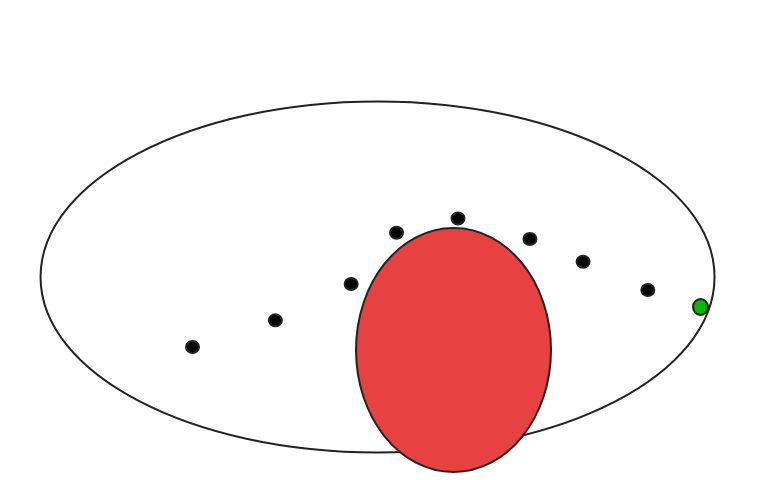
\includegraphics[width=200px]{images/infeasible_constraint.png}
% %\end{center}
% 
% If the runtime of the simulation depends on its inputs, and the simulation is not allowed to finish when a runtime threshold is met, the runtime will force some inputs to be infeasible.
% However, when the simulation does complete, its runtime is quantifiable, and can be used to construct a model of the infeasible region.
% An algorithm that wishes to minimize this simulation is forced to account for this constraint.
% 
% 
% An always feasible algorithm is also an \emph{any-time} algorithm.
% Anytime algorithms are a class of algorithms that can conveniently be run as long as desired and return the best solution found so far if interrupted.
% These algorithm are of practical importance when problems have uncertain time complexity.
% 


\section{Background}

\subsection{Notation}

Any variables that depend on the iteration will be super-scripted by $k$.
For example, the $k$-th iterate is given by $\iteratek$, and the model of the objective is given by $\modelk$.
The $i$-th row of the matrix $A$ is denoted $A_i$, while the $i$-th column is denoted $A_{\bullet i}$.
Subscripts on vectors are used as an index into the vector, while vectors in a sequence of vectors use superscripts.
Matrices are denoted with capital letters, and we use $e_i$ to denote the $i$-th unit vector.                     %, while sets are denoted with capital italic letters.

$B_k(c; \Delta)$ is the ball of radius $\Delta$ in the $k$ norm, centered at point $c$ .
$\delta_{i,j}$ is the kronecker delta, $\delta_{i,i} = 1$, $\delta_{i,j} = 0$ if $i\ne j$.


\subsection{Model-based Trust Region Methods}

We will modify the following derivative free trust region algorithm.
%A set of poised points are chosen for some radius $\Delta_k>0$ about the current iterate.
The objective value and derivatives are approximated in a trust region around the current iterate to construct their model functions.
Next, this model function is minimized over the trust region and the minimum argument becomes the trial point.
The objective is evaluated at the trial point and a measure of reduction $\rho$ is computed.
If $\rho$ implies that sufficient reduction has been made and that the model approximates the function well, the trial point is accepted as the new iterate.
Otherwise, the trust region is reduced to increase model accuracy.
The algorithm terminates when both and a criticality measure $\chik$ and the trust region radius $\Delta_k$ reach sufficiently small thresholds of $\tau_{\chi}$ and $\tau_{\Delta}$.


For unconstrained optimization, the algorithmic framework is described in \cref{unconstrained_dfo}.
% 	\begin {itemize}
%         \item The objective is evaluated at a set of sample point $Y$ to approximate $f$ \cref{interpolation}
%         \item Geometric properties ensure bounds on $f(x) - \modelk(x)$, $\nabla f(x) - \gradmodelk(x)$, and $\nabla^2 f(x) - \nabla^2\modelk(x)\;\forall x$ in the trust region \cref{geometry}
% 		%\[
% 		%\modelk(x) = f(\iteratek) + \nabla f(\iteratek)^T (x-\iteratek) + \frac 1 2 (x-\iteratek)^T\nabla^2f(\iteratek)(x-\iteratek)
% 		%\]
% 		\item If $\rho$ is large, $\iteratekpone=\iteratek+\trialk$ (accept) and either increase the radius or decrease if $\nabla \modelk(\iteratek)$ is small
% \end{itemize}

\begin{algorithm}[H]
    \caption{Unconstrained Derivative Free Algorithm}
    \label{unconstrained_dfo}
    \begin{itemize}
        \item[\textbf{Step 0}] \textbf{(Initialization)} \\
            Initialize tolerance constants $\tau_{\chi} \ge 0$, $\tau_{\Delta} \ge 0$, starting point $x^{(0)}$, initial radius $\Delta_0 > 0$, iteration counter $k=0$, and constants $\omegadec \in (0, 1)$, $ \gammasm \in (0, 1)$, $\gammabi \in (\gammasm, 1)$.
            
        \item[\textbf{Step 1}] \textbf{(Construct the model function)} \\
            Call the model improvement ``\cref{model_improving_algorithm}" to provide a set of sample points $Y^{(k)}$.
            Evaluate the objective on these points and use interpolation \cref{interpolation_formula} to construct the model function $\modelk(x)$.
        
        \item[\textbf{Step 2}] \textbf{(Check stopping criteria)} \\
            Compute the criticality measure $\chik$ such as $\chik = \|\nabla\modelk(\iteratek)\|$. \begin{itemize}
                \item[] If $ \chik < \tau_{\chi} $ and $\Delta_k<\tau_{\Delta}$ then return solution $\iteratek$.
                \item[] If $ \chik < \tau_{\chi} $ but $\Delta_k\ge\tau_{\Delta}$ then  
                set $\Delta_{k+1} \gets \omegadec\Delta_{k}$, 
                $x^{(k+1)} \gets \iteratek$,
                $k \gets k+1$ and go to Step 1.
            \end{itemize}
        
        \item[\textbf{Step 3}] \textbf{(Solve the trust region subproblem)} \\
            Compute $\trialk = \argmin_{s\in B_2(0; \Delta_k)} \modelk (\iteratek + s)$ where $B_2(0; \Delta_k)$ is the ball of radius $\Delta_k$ defined in \cref{tab:TableOfNotation}.
            
        \item[\textbf{Step 4}] \textbf{(Test for improvement)} \\
            Compute $\rho$ with \cref{rho} \begin{itemize}
                \item[] If $\rho < \gammasm$ then $\iteratekpone \gets \iteratek$ (reject) and $\Delta_{k+1} \gets \omegadec\Delta_{k}$
                \item[] If $\rho \ge \gammasm$ and $\rho < \gammabi$ then $\iteratekpone\gets\iteratek+\trialk$ (accept) $\Delta_{k+1} \gets \omegadec\Delta_{k}$
                \item[] If $\rho \ge \gammabi$ and $\|\trialk\| = \Delta_{k}$ then $\iteratekpone=\iteratek+\trialk$ (accept) $\Delta_{k+1} \gets \omegainc\Delta_{k}$
                % and either increase the radius or decrease if $\nabla \modelk(\iteratek)$ is small
            \end{itemize}
            $k \gets k+1$ and go to Step 1.
    \end{itemize}
\end{algorithm}

This derivative-free optimization algorithm differs from the classical trust region algorithm in two important respects:
\begin{enumerate}
    \item Models are constructed without derivative information.
    \item The trust region radius $\Delta_k$ must go to zero as $k\to\infty$.
\end{enumerate}

This is required to ensure that the gradient of the model function is equal to the gradient of $f$ in the limit.
Our goal is to generalize this framework to handle constraints, where we must ensure no constraint violation occurs while also ensuring the accuracy of the models of the constraints.
% Two challenges while adopting this framework to derivative free optimization are
% 
% Because explicit derivatives are not available, Taylor approximations cannot be used.
% The alternative to Taylor approximations that we employ is interpolation.
% Also, classical trust region methods do not require $\Delta_k \to 0$, but the bounds on model accuracy in derivative free optimization depend on the trust region radius.
% This means that in order to ensure $\nabla f < c\tau$ using the approximation  $\nabla \modelk < \tau$, the trust region must be sufficiently small.
%   
  

\section{Derivative Free Background}
% 
% \subsection{Strategy}
% A reasonable approach to DFO is to modify classical algorithms that rely on derivatives by using the derivatives of the model functions whenever a derivative is needed in the algorithm.
% However, the lack of explicit derivatives pose several challenges, which necessitate changes in the classical algorithms.
% First, care must be taken to ensure that the model functions are sufficiently accurate approximations to the true functions.
% This means that geometry of the sample points must be considered.
% It also means that the trust-region radius must get arbitrarily small.
% 
% The transition to the derivative-free setting also provides some interesting research opportunities.
% In particular, because function evaluations are so costly, there is potential for significant gains by considering more complex optimization paradigms.
% For example, Sequential Quadratic Programming (SQP) methods use subproblems involving quadratic approximations of the objective function $f$ and linear approximations of the constraint functions.
% In the derivative-free setting, it may be worthwhile to explore other variations of the classical algorithms.
% For example, it might be worthwhile to construct quadratic models of the constraint functions, which might result in fewer iterations overall.
% 
% It might also be worthwhile to consider using different sample sets for fitting different functions.  
% For example, the SQP trust-region filter method involves constructing a quadratic model of the objective function and linear models of the constraint functions.  But this raises an interesting question, since a good sample set for constructing a quadratic model may not be ideal for fitting the linear functions modeling the constraints.  

\subsection{Recent Work}
\paragraph{Applications}
Recently, there has been a growth in applications of derivative free optimization.
Such applications include photo-injector optimization \cite{1742-6596-874-1-012062}, circuitry arrangements \cite{PLOSKAS201816}, machine learning \cite{KS2018}, volume optimization \cite{Cheng2017}, and reliability based optimization \cite{Gao2017}.

\paragraph{Constrained derivative free algorithms}
To address the rise in these applications, new algorithms are being developed such as \cite{doi:10.1080/10556788.2015.1026968} which is an algorithm similar to the one presented here, but the sample points are not always feasible.
\cite{Troltzsch2016} presents another similar algorithm for equality based constraints.
\cite{infeasiblestarting} presents an algorithm which accepts an infeasible starting point.
\cite{Gao2018} also presents an algorithm for linearly constrained derivative free optimization that uses a backtracking technique to minimize the number of evaluations required.

\paragraph{Subproblems}
Some work has been done within trust region algorithms to improve the update policy \cite{Kamandi2017}.
Also, \cite{Verderio2017} and \cite{doi:10.1080/10556780802409296} discuss geometric conditions of the sample points required for global convergence.
Finally, \cite{AMAIOUA201813} uses a mesh adaptive search to solve quadratic subproblems.


\paragraph{Complexity Analysis}

A derivation is found in \cite{doi:10.1137/151005683} which shows that to driver the norm of the gradient less than $\epsilon$, the number of function evaluations can be bounded by $O(\epsilon^{-2})$ 
%and $O(n^2\epsilon^{-2})$ 
function evaluations for derivative free model based approaches. Also, cubic over estimation with finite differences can acheive $O(\epsilon^{-1.5})$. \cite{doi:10.1093/imanum/drx043} is another recent paper presenting complexity analysis using probabilistic methods.


\paragraph{Reviews}
Within \cite{DUMMY:intro_book} derivative-free methods are developed in detail.
This is the first text book devoted to derivative free optimization.
It contains a good explanation of ensuring geometry of the current set with poisedness for unconstrained problems and also covers other derivative-free methods including direct-search and line search.

A good review of derivative free algorithms and software libraries can be found in \cite{DUMMY:review}.
This compares several software libraries, and reviews the development of derivative free optimization since it started.
Another recent review can be found in \cite{DUMMY:review2} and \cite{Larson_2019}.

% TODOOOOOOOOOOOOOOOOOOOOOOOOOOOOOOOOOOOOOOOOOOOOOOOOOOOOOOOOOOOOOOOOOOOOOOOOOOOOOOOOOOOOOOOOOOOOOOOOOOOOOOOOOOOO
% READ THIS


\subsection{Sample Set Geometry}
\subsubsection{Interpolation}
\label{interpolation}

Derivative free trust region methods construct model functions from a family of functions spanned by a set of $p \in \mathbb N$ basis functions  $\{\phi_0, \phi_2, \ldots, \phi_p\}$.
Each member of this family has the from $\modelk(x) = \sum_{i=0}^p\alpha_i\phi_i(x)$ for some scalar coefficients $\alpha_i, i \in \{0, \ldots, p\}$.

In our method, we use interpolation to choose the coefficients so that $\modelk$ agrees with $f$ on a set of $p+1$ sample points $Y = \{y^0, y^1, \ldots, y^p\}$ for which the functions have been evaluated.
Thus the model functions must satisfy:
\begin{align}
\label{interpolation_condition}
\modelk(y^i) = f(y^i) \quad \forall \quad 0 \le i \le p.
\end{align}
This is known as the \emph{interpolation condition}.

To satisfy the interpolation condition \cref{interpolation_condition}, we then chose this linear combination by selecting coefficients $\alpha_0, \ldots, \alpha_p$ to satisfy
\begin{align}
\label{interpolation_formula}
    \modelk(y^i) = \sum^p_{j=0}\alpha_j\phi_j(y^i) = f(y^i) \quad \forall \quad 0 \le i \le p.
\end{align}

% We can also write this equation in matrix form.
If we define the Vandermode matrix as
\begin{align}
\label{vandermonde}
V=
\begin{bmatrix}
    \phi_0(y^0)      & \phi_1(y^0)       & \ldots & \phi_{p}(y^0)      \\
    \phi_0(y^1)      & \phi_1(y^1)       & \dots  & \phi_{p}(y^1)      \\
                     &                   & \vdots &                    \\
    \phi_0(y^{p})    & \phi_1(y^{p})     & \ldots & \phi_{p}(y^{p})
\end{bmatrix},
\end{align}

the interpolation condition becomes:
\begin{align}
\label{matrix_form}
V
\begin{bmatrix}
    \alpha_0     \\
    \alpha_1     \\
    \vdots       \\
    \alpha_p
\end{bmatrix}
=
\begin{bmatrix}
    f(y^0)     \\
    f(y^1)     \\
    \vdots     \\
    f(y^p)
\end{bmatrix}
\end{align}

% Suppose that we use $p+1$ sample points $Y = \{y^0, y^1, \ldots, y^p\}$ to construct the approximation of $f$.
We desire a method for choosing these sample points that provides error bounds on not only the function values, but also on orders of derivatives in some region around the current iterate.
% The model is constructed to agree with the original functions on at least the sample points: we evaluate the objective here, so that we know the true function values at these points.
% For the objective, this becomes

%It is convenient to write the model as a linear combination of basis polynomials $\{\phi_0, \phi_2, \ldots, \phi_p\}$.


\subsubsection{Geometry}
\label{geometry}
The term \emph{geometry} describes how the distribution of points in the sample set $Y$ affects the model's accuracy.
\cref{matrix_form} has a unique solution if and only if $V$ is nonsingular, in this case, we say that the sample set $Y$ is \emph{poised} for interpolation with respect to the basis functions $\phi_i$.
However, even when $V$ is nonsingular but ``close" to singular, as measured by its condition number, the model's approximation may become inaccurate.
% The condition number of $V$ measures how far the current Vandermode matrix is from being illpoised.
Algorithms must be careful to avoid choices of sample points $Y$ that cause the condition number of this matrix to be too large.

In the case of polynomial model functions, a careful analysis of model accuracy can be performed using \emph{Lagrange polynomials}.
Let the space of polynomials with degree less than or equal to $d$ be denoted $\polydn$ and have dimension $p+1$.
The Lagrange polynomials $l_0, l_1, \ldots, l_p$ for the sample set $Y$ are a basis of $\polydn$ such that
\[
l_i(y^j) = \delta_{i,j}
\]
where $\delta_{i,j} = \{0 \;\text{if}\; i\ne j,\quad 1 \;\text{if} \; i = j \}$ is the Kronecker-delta function.
%For example, after this change of basis, note that the Vandermonde matrix becomes the identity matrix.
Thus, we can conveniently write
\[
\label{reg}
\modelk(x) = \sum^p_{j=0}f(y^i)l_i(x).
\]
%This implies computing the change of basis to the Lagrange polynomials amounts to inverting this Vandermonde matrix.
%This relationship allows us to use properties of the Vandermonde matrix and these Lagrange polynomials to find conditions on our sample points that ensure nice geometry.

We say that a set $Y$ is \emph{$\Lambda$-poised} for a fixed constant $\Lambda$ with respect to a bases $\phi$ on the set 
$B \subset \mathbb R^n$ if and only if for the Lagrange polynomials $l_i$ associated with $Y$
\begin{align}
\Lambda \ge \max_{0\le i\le p}\max_{x\in B}|l_i(x)|.
\end{align}

% This can be shown to be equivalent to the following condition \cite{DUMMY:intro_book}.
% For any $x \in B_2(0, 1)$ there is a $\lambda \in \mathbb R ^ {p+1}$ such that 
% \begin{align}
% \sum_{i=0}^p\lambda_i\phi_i(y^i) = \phi(x) \\
% \|\lambda\|_{\infty} \le \Lambda.
% \end{align}

% This can ensure that the Vandermonde matrix is well conditioned.
This is useful because of the following results \cite{DUMMY:intro_book}:
Assuming that $f$ is twice continuously differentiable in an open domain containing $B_2(y^0, \Delta)$ and has a Lipschitz continuous Hessian, using quadratic interpolation there exist constants $\kappa_{ef}, \kappa_{eg}$, and $\kappa_{eh}$ depending only on the dimension and Lipschitz constant of $\nabla^2 f$ such that for any $y \in B_2(y^0, \Delta)$ :
\begin{align}
 \label{fully_quadratic}
 \|f(y) - \modelk(y)\| \le \kappa_{ef} \Lambda \Delta^3 \\
 \|\nabla f(y) - \nabla \modelk(y)\| \le \kappa_{eg} \Lambda \Delta^2 \\
 \|\nabla^2 f(y) - \nabla^2 \modelk(y)\| \le \kappa_{eh}\Lambda \Delta .\\
\end{align}
\cite{DUMMY:intro_book} also shows that ensuring a bound on the condition number of the Vandermonde matrix ensures $\Lambda$-poisedness.

In particular, these bounds ensure that the following accuracy condition is satisfied, which is used by \cite{Conejo:2013:GCT:2620806.2621814} to prove convergence to a first order critical point: 
\begin{equation}
\label{accuracy}
\|\nabla \modelk(\iteratek) - \nabla f(\iteratek) \| \le \kappa_g \Delta_k
\end{equation}
 for some fixed constant $\kappa_g$ independent of $k$.
We will extend these results for ellipsoidal trust regions in \cref{ellipsoidal_lambda}.
 

%used to find the coefficients $\lambda$ to express the model function in terms of a basis of Lagrange polynomials $l_i$
The following example illustrates how interpolating with an ill-poised set can produce an inaccurate model.
% Problems become apparent when comparing the Lagrange polynomials associated with a poised set with those of an ill poised set.
In \cref{pvip}, a set of quadratic polynomials is used to interpolate the function $f(x) = 5 + x + y + (x + y) ^ 2 - \frac 1 {250} y ^ 4$.
We can see that the difference between the model and $f$ are much larger when the points are chosen to be nearly collinear.
This results in a much higher $\Lambda$.

\begin{figure}[h]
    \centering
    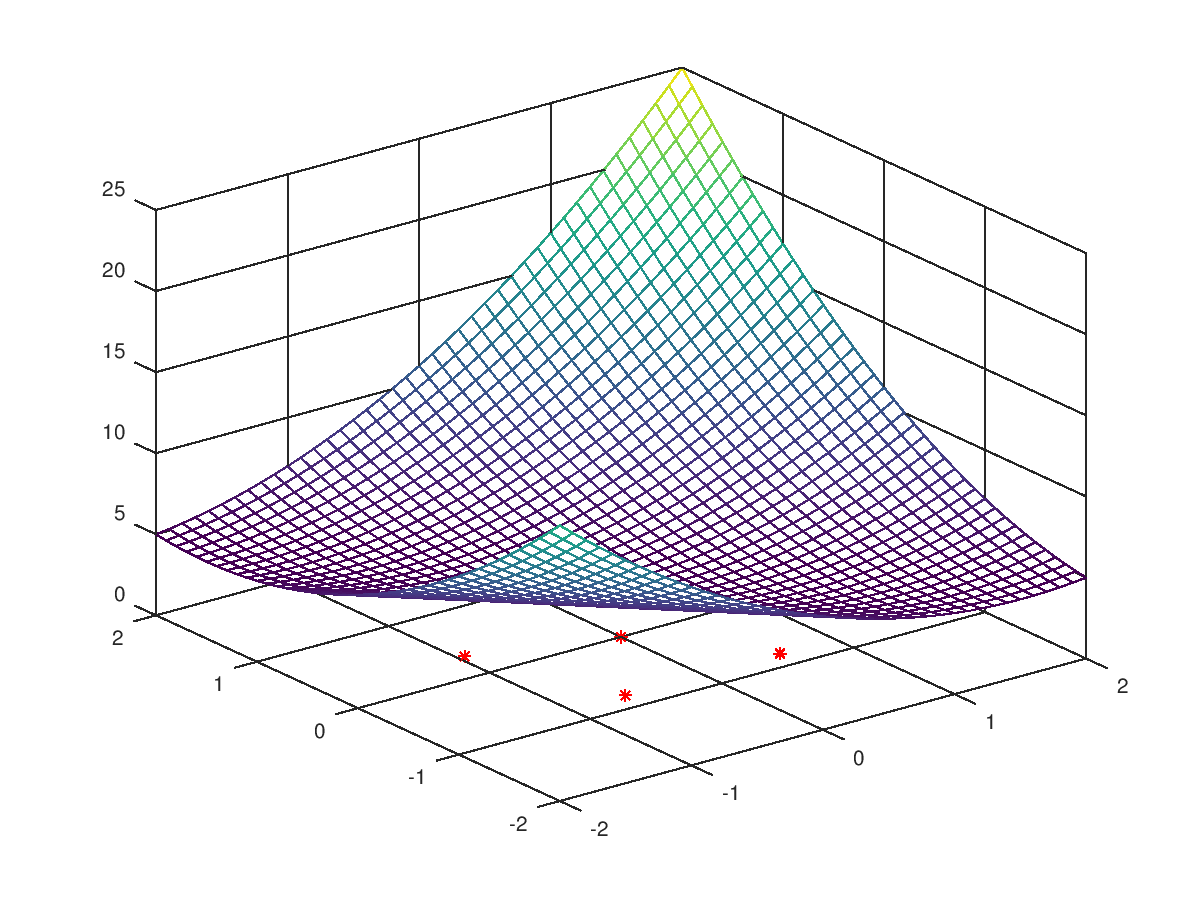
\includegraphics[width=200px]{images/poised_good.png}
    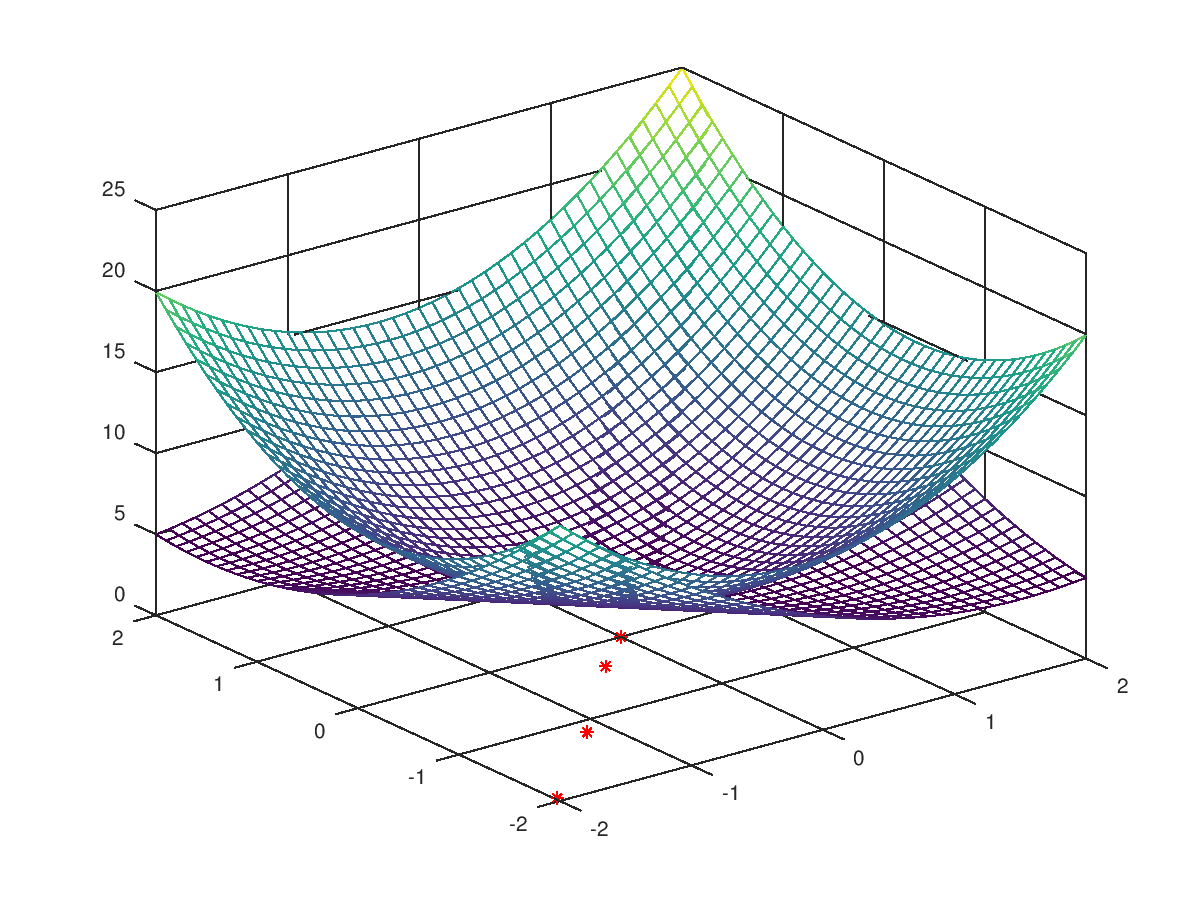
\includegraphics[width=200px]{images/poised_bad.png}
    \caption{
		Poised vs Ill poised.
		On the left, a well poised sample set is used and the model is indistinguishable from the true function.
		On the right, the sample set has poor geometry, and the model goes above the true function.
	}
    \label{pvip}
\end{figure}


A more detailed discussion can be found in \cite{doi:10.1080/10556780802409296}, but a step to ensure good geometry is required for convergence analysis although it may come at the expense of adding more function evaluations.

\subsubsection{Geometry Ensuring Algorithms}

Sample points are chosen by a geometry ensuring algorithm.
At any given time, the algorithm has evaluated 1 or more sample points.
Initially, only the starting point $x_0$ is evaluated, so that points must be added to the sample set.
Evaluated points within the trust region should be reused when possible, but the algorithm may have to replace some points to ensure a well poised set on the new trust region.
We call the algorithm that adds points, replacing where necessary, the \emph{model improvement algorithm}.
One classic such algorithm is presented in \cite{DUMMY:intro_book}.

The idea behind this algorithm is to perform an LU factorization with partial pivoting on the Vandermonde matrix.
As we have seen, this computes the basis for the Lagrange polynomials corresponding to $Y$.
However, when this LU factorization encounters a small pivot, the point corresponding to that row is replaced, improving the condition number of the Vandermonde matrix.

In practice, we first shift the sample set $Y$ by subtracting the current iterate and dividing by the trust region radius:
\begin{align}
\bar{Y} = [0, \frac{y^1 - y^0}{\Delta}, \ldots, \frac{y^p - y^0}{\Delta}]
\end{align}

At times, the algorithm will not have all $p+1$ points.
This can be because it is only given one point during initialization, or because points not within the trust region are removed.
Because the model improvement algorithm requires all $p+1$ points, we initialize $y^i = y^0$ for any $0 < i \le p$ corresponding to a missing point.
We choose a threshold $0 < \ximin < 1$, and follow \cref{model_improving_algorithm}:

\begin{algorithm}[H]
    \caption{Model Improvement Algorithm}
    \label{model_improving_algorithm}
    \begin{itemize}
        \item[\textbf{Step 0}] \textbf{(Initialization)} \\
            Initialize $i=1$.
            Given a non-empty set $Y$ of $p+1$ points. 
            Construct the Vandermonde matrix $V_{i,j} = \phi_j(\frac 1 {\Delta}(y^i - y^0))$.
			Initialize constant $\ximin > 0$.
        \item[\textbf{Step 1}] \textbf{(Pivot)} \\
            Swap row $i$ with row $i_{\max} = \arg \max_{j|j\ge i} V_{j,i} $
        
        \item[\textbf{Step 2}] \textbf{(Check threshold)} \begin{itemize}
                \item[] If $|V_{i,i}| < \ximin$ then select \label{next_point} $\hat y = \argmax_{t | \|t\|\le 1} |\phi_i(t)|$
                \item[] Replace row $i$ with $V_{i, j} \gets \phi_j(\hat y)$.
            \end{itemize}
        
        \item[\textbf{Step 3}] \textbf{(LU)} \begin{itemize}
                \item[] Set $V_i \gets \frac{1}{V_{i,i}} V_i$
                \item[] Set $V_{\bullet j} \gets V_{\bullet j} - V_{i,j} V_{\bullet j} \forall j=i \ldots p$
            \end{itemize}
            If $i = p$ then \textbf{Stop}, otherwise Set $i \gets i+1$ and go to Step 1
    \end{itemize}
\end{algorithm}
% 
% \paragraph{Proximity}
% 
% Proximity refers to the trust region radius.
% The trust region must go to zero if we are to be sure we have reached a critical point.
% In general, the smaller the trust region, the closer to linear or quadratic the original function will look.
% This is because the model's error term is proportional to the trust region radius.
% 
% In classical trust region algorithms, there is no need for the trust region radius to go to zero.
% Therefore, extra care must be taken to ensure this while modifying such algorithms.


% \begin{algorithmic}
% \If{$\rho < \gamma_1$}
%     \State $\iteratekpone \gets \iteratek$ (reject)
%     \State $\Delta_{k+1} \gets \omega_{\text{dec}} \Delta_k$
% \ElsIf{$\gamma_1 \le \rho \le \gamma_2$}
%     \State $\iteratekpone\gets \gets \iteratek + \trialk$ (accept)
%     \State $\Delta_{k+1} \gets \omega_{\text{dec}} \Delta_k$
% \ElsIf {$\rho > \gamma_2$}
%     \State $\iteratekpone \gets \iteratek + \trialk$ (accept)
%     \If
%         \State $\Delta_{k+1} \gets \omega_{\text{dec}} \Delta_k$
%     \Else
%         \State $\Delta_{k+1} \gets \omega_{\text{inc}} \Delta_k$
%     \EndIf
% \EndIf
% \end{algorithmic}


\subsection{Algorithm Components}




We will discuss several building blocks of the algorithm before going into the algorithm's detail.




\subsubsection{Criticality Measure}

In order to define stopping criteria for the algorithm, we introduce a criticality measure $\chi$ which goes to zero as the iterates approach a first order critical point.
When the criticality measure is small, we must also decrease the trust region radius.
Once this has reached a small enough threshold $\tau_{\chi}$ and the trust region is small enough ($\Delta_k < \tau_{\Delta}$), we can terminate the algorithm.
For now, our algorithm is designed to work with convex constraints, so we employ a classic criticality measure discussed in \cite{ConnGoulToin00} of

\[
\chik = \|\iteratek - \text{Proj}_{\feasiblek}(\iteratek- \nabla \modelk(\iteratek))\|
\]
where $\feasiblek$ denotes the feasible region: $\feasiblek = \{x \in X | \modelconstrainti(x) \le 0 \quad \forall i \in \mathcal I \wedge c_i(x) = 0 \quad \forall i \in \mathcal E \}$.
This criticality measure measures how far the current is from satisfying the first order optimality conditions for $\iteratek$ to be a constrained minimum of $\modelk$.
When $ \lim_{k\to\infty} \chik = 0$, $\lim_{k\to\infty}\Delta_k = 0$, and $\lim_{k\to\infty}\iteratek = x^{\star}$, then we have that $x^{\star}$ also satisfies the first order optimality conditions of being a constrained minimum of $f$.

%we have $x = \text{Proj}_{\feasiblek}(x - \nabla \modelk(x))$ so that

$\chik$ can be computed as 
\begin{align}
\label{critical}
\trialk = \min_{s \in \feasiblek} \|\iteratek - \nabla \modelk(\iteratek) - s\|^2 \\
\chik = \|\iteratek - \trialk \|^2 \\
\end{align}

% This remains large while there is feasible search space along a descent direction, but small otherwise or if the gradient goes to zero.

% Namely, when $ \chik(x) = 0$, we have $x = \text{Proj}_{\feasiblek}(x - \nabla \modelk(x))$ so that there is no decent direction along $\nabla \modelk(x)$ as it points away from the feasible region.
% As $\Delta_k$ gets smaller, we also have that $\modelk$ better represents $\nabla f$, so that $\nabla f$ will also either be zero or lie in the iterate's normal cone.

\subsubsection{Assessing Model Accuracy and Radius Management}

Each iteration that evaluates a trial point must also test the accuracy of the model functions.
To test the accuracy, we calculate a quantity
\begin{equation}
\label{rho}
\rho_k = \frac{f(\iteratek) - f(\iteratek+\trialk)}{\modelk(\iteratek) - \modelk(\iteratek+\trialk)}
\end{equation}
which measures the actual improvement over the predicted improvement.
A small $\rho_k$ implies the model functions are not sufficiently accurate.
Values of $\rho_k$ close to $1$ imply that the model accurately predicted the new objective value.
A large $\rho_k$ implies progress minimizing the objective although the model was not accurate.
This has been widely used within trust region frameworks such as \cite{Conn:2000:TM:357813} and within a derivative free context \cite{DUMMY:intro_book}.
The user supplies fixed constants $0 < \gammasm \le \gammabi \le 1$ as thresholds on $\rho_k$ and $0 < \omega_{\text{dec}} < 1 \le \omega_{\text{inc}}$ as decrement or increment factors to determine the trust region update policy.
The update policy frequently follows Step 4 within algorithm \cref{unconstrained_dfo} repeated within \cref{trust_region_update} for ease.

\begin{algorithm}[H]
    \caption{Trust Region Update Policy}
    \label{trust_region_update}
    \begin{itemize}
        \item[\textbf{Step 4}] \textbf{(Test for improvement)} \\
            Compute $\rho_k$ with \cref{rho} \begin{itemize}
                \item[] If $\rho_k < \gammasm$ then set $\iteratekpone \gets \iteratek$ (reject) and $\Delta_{k+1} \gets \omegadec\Delta_{k}$
                \item[] If $\rho_k \ge \gammasm$ and $\rho < \gammabi$ then set $\iteratekpone\gets\iteratek+\trialk$ (accept) and $\Delta_{k+1} \gets \omegadec\Delta_{k}$
                \item[] If $\rho_k \ge \gammabi$ and $\|\trialk\| = \Delta_{k}$ then set $\iteratekpone=\iteratek+\trialk$ (accept) and $\Delta_{k+1} \gets \omegainc\Delta_{k}$
                % and either increase the radius or decrease if $\nabla \modelk(\iteratek)$ is small
            \end{itemize}
            $k \gets k+1$ and go to Step 1.
    \end{itemize}
\end{algorithm}

\subsubsection{Sufficient Model Reduction}

To ensure sufficient reduction of the objective's model function during each iteration, we impose the following efficiency condition:
\begin{equation}
\label{efficiency}
\modelk(\iteratek) - \modelk(\iteratek + \trialk) \ge \kappa_f \chi_k \min\left\{ \frac{\chi_k}{1+\|\nabla^2 \modelk(\iteratek)\|}, \dk, 1 \right\}
\end{equation}
where $\kappa_f$ is a constant independent of $k$.
This is widely used within trust region frameworks such as \cite{Conejo:2013:GCT:2620806.2621814} and \cite{Conn:2000:TM:357813}.
It can be shown that the \emph{generalized Cauchy point} satisfies this condition \cite{Conn:2000:TM:357813}.


\subsubsection{Trust Regions}
Our algorithm maintains up to three trust regions.
The outer trust region is an $L_1$ ball of radius $ \dk $ defined by
\begin{equation}
\label{trust_region}
\outertrk = B_{\infty}(\iteratek,\dk) = \{x\in \mathbb R^n | \; {\iteratek}_i - \dk \le x_i \le {\iteratek}_i + \dk \quad \forall 1\le i \le n\}.
\end{equation}

Note that the outer trust region may include infeasible points.
To ensure feasibility of all sample points, we construct an inner trust region for sample points $ \sampletrk $  satisfying 
$\sampletrk \subset \outertrk \cap \feasiblek$ and $\iteratek \in \sampletrk $.
However, we do not want to limit the search for a new iterate to the same trust region we use to construct the model.
This means we introduce another trust region $ \searchtrk $ that also satisfies $ \searchtrk \subset \outertrk \cap \feasiblek$ and $\iteratek \in \searchtrk $ for the trust region subproblem.


We consider general strategies for constructing $ \sampletrk $ and $ \searchtrk $.
\begin{itemize}
\item[1.] Take $\label{redpill} \sampletrk = \searchtrk = \outertrk \cap \feasiblek $. This results in a polyhedral trust region, so we refer to this approach as the \emph{Polyhedral Trust Region Approach}.
% \item[2.] Let $\label{hybrid} \sampletrk \subseteq \searchtrk = \outertrk \cap \feasiblek $ where $\sampletrk$ has an ellipsoidal shape. This is referred to as the \emph{Hyrbid Trust Region Approach}
\item[2.] Force $\label{bluepill} \sampletrk \subseteq \searchtrk \subseteq \outertrk \cap \feasiblek $ where $\sampletrk$ has an ellipsoidal shape. This is referred to as the \emph{Ellipsoidal Trust Region Approach}
\end{itemize}

The advantage of the ellipsoidal trust region approach \cref{bluepill} is that we can reuse classical methods for ensuring good geometry.
We can construct $\sampletrk$ to be ellipsoidal and use efficient algorithms within \cite{DUMMY:intro_book} to satisfy \cref{accuracy}.
However, we must be careful while choosing $ \searchtrk$ to allow sufficient reduction when we solve the trust region subproblem using the inner trust region.
The search trust region is used while selecting the next iterate:
\begin{align*}
\trialk = \argmin_{\trialk \in \searchtrk} \modelk(\iteratek + \trialk)
\end{align*}

\label{which_trust_region}
When using the ellipsoidal trust region approach, we have two choices for this trust region:
\begin{align}
\searchtrk = \sampletrk \label{search_a_little}
\end{align}
\begin{align}
\searchtrk = \outertrk \cap \feasiblek \label{search_a_lot}
\end{align}
Namely, in \cref{search_a_little} with an ellipsoidal inner trust region, we still have an option to select our trial point from the entire $\trialk \in \outertrk \cap \feasiblek$.

To complete the polyhedral trust region approach \cref{redpill}, %$\innertrk = \outertrk \cap \feasiblek$
, we need some redefinition of poisedness for polyhedral shapes.
However, since the trust region is larger, it is easier to ensure sufficient reduction.
This strategy has the drawback that it will yield sample points close to the boundary of the feasible region.
This may cause more infeasible evaluation attempts when we use models to approximate black-box constraints this may.

The classical methods for ensuring good geometry require an optimization call to the model functions over a sphere.
This is no longer possible in the polyhedral trust region approach.
However, the bounds produced over the entire trust region may also be stronger than required as the models will only be used on the feasible region.
This may mean the geometric requirements can be reduced.
Looking again at the ill-poised set in \cref{aoip}, the set of nearly collinear sample points actually does appear to be accurate over a smaller trust region.


\begin{figure}[h]
    \centering
    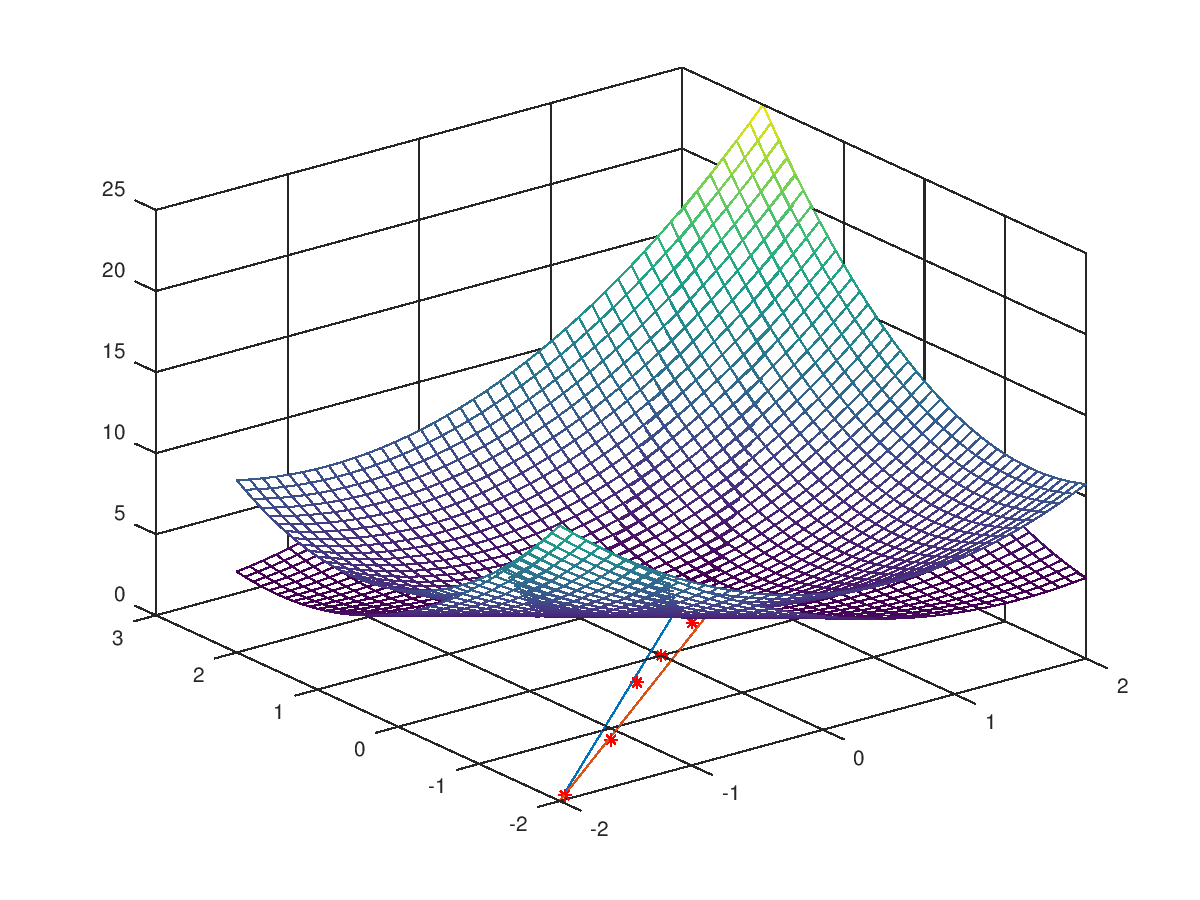
\includegraphics[width=200px]{images/poised_bad_but_good.png}
    \caption{Accurate model over thin trust region from illpoised set}
    \label{aoip}
\end{figure}


Within our algorithm, if $ \outertrk \subseteq \feasiblek$ we can set $ \sampletrk $ to be a sphere.
This saves the computation of $ \sampletrk $ when it is not needed, as there are no nearby constraints.




% \paragraph{}
% While including a center search and only using a sphere for $\sampletrk$ ensures that this will be the case as long as there is an interior point to the feasible region.
% However, for more complicated ellipsoid searches must be able to find an ellipse.
% One strategy that ensures the ellipse can be constructed for all of our ellipse searches is to find an ball containing the current iterate and running a local search optimization routine with this initial ball as input.


% 
% \paragraph{}
% Another strategy is to add a check within the \emph{ConstructTrustRegion} routine that decreases the trust region radius whenever a suitable ellipse is not found.
% The presented convergence analysis will still hold as $S$ can contain only finitely many terms not in $\bar S$.

% \paragraph{}
% \color{red}
% For convex constraints, there will exist a bound on the condition numer of $\qk$ as long as $\outertrk$ is bounded.
% An argument for this might be as follows:
% Maybe, by increasing the outer trust region radius, we can only increase the condition number of $\qk$.
% \color{black}






\section{Algorithms}


\subsection{Using full models}
I have implemented an algorithm that uses higher order models to approximate the constraints.

In this algorithm, we add additional degrees of freedom to the constraints to cut off points that have been evaluated and are infeasible.
The models are forced to be a given negative value at these points.

One question for this method is how many constraints to model.


I implemented Kriging, as this can use as many points as are available.
However, this requires using some artificial value of the constraints at infeasible points.

\subsection{Using linear models}

Another method is to add additional linear constraints each time a new point is evaluated and infeasible.

Each new linear constraint cuts off an infeasible point and stays atleast a fraction of the trust region away from that infeasible point.


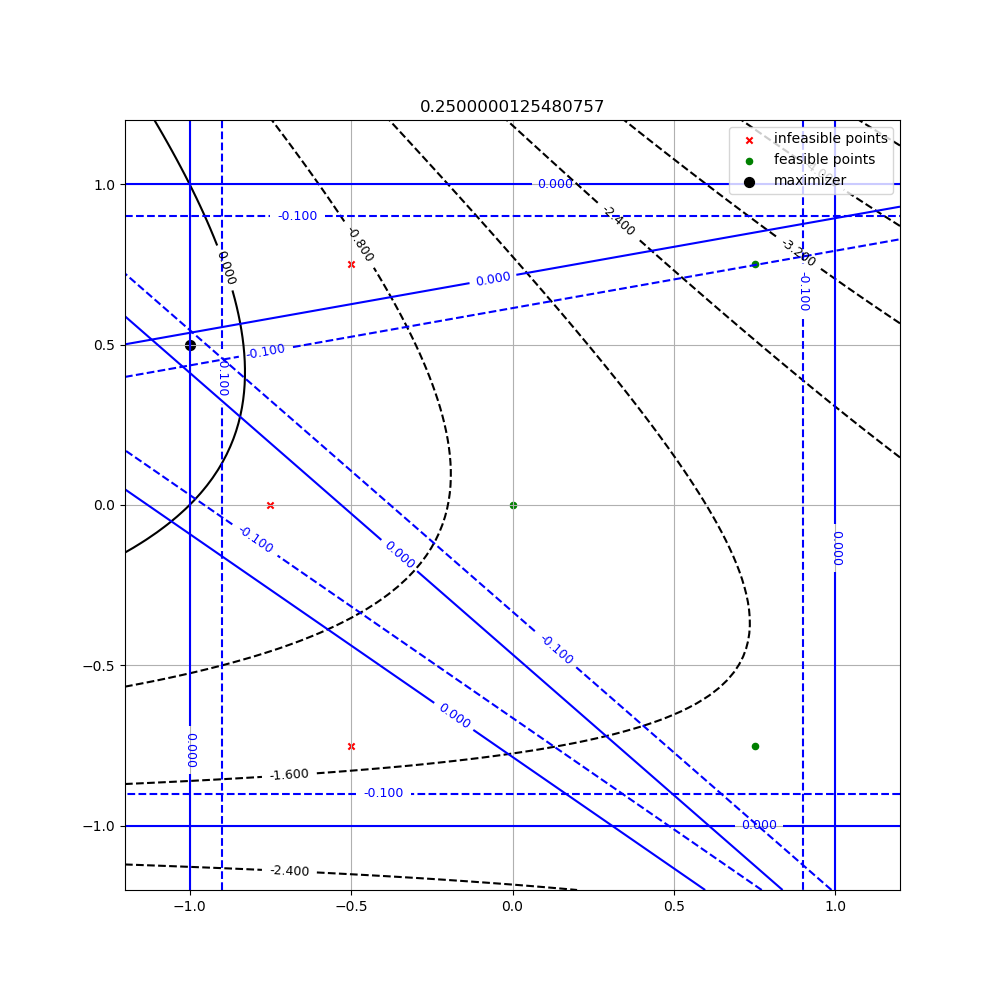
\includegraphics[width=300px]{images/pyomo_cut_solution.png}

\subsubsection{formulation}

The optimization program for finding this constraint is given by:

A set of $u^i, 1 \le i \le n_{I}$ infeasible points.
A set of $v^i, 1 \le i \le n_{F}$ feasible points.

The current Lagrange polynomial $\frac 1 2 x^T Q x + b^Tx$.
Require all infeasible point to be a distance at least $d$ from the feasible region.


Find a set of planes $(n^i, b^i), 1 \le i \le n_{P}$.

Require $n_P \ge n_I$.


What we want big:
\begin{align}
\max_{x} & \frac 1 2 x^T Q x + b^Tx &\\
 & {n^i}^T x \le b^i & \forall 1 \le i \le n_{P} \\
 & {n^i}^T v_j \le b^i & \forall 1 \le i \le n_{P}, 1\le j\le  n_{F} \\
 & {n^i}^T u_i \ge b^i + d & \forall 1 \le i \le n_{I} \\
 & \| n^i \| = 1 & \forall 1 \le i \le n_{I} \\
 & 0 \le x_i \le 1 & \forall 1 \le i \le n \\
\end{align}


A set of $v_i, 1 \le i \le n_{I}$ feasible points.




\subsection{Using a sacred region}


\begin{itemize}
    \item Define a suitable ellipsoid to be an ellipsoid that satisfies the following conditions: \begin{itemize}
        \item It can be scaled by a factor of 2 to include the current iterate.
        \item It touches a boundary of the current trust region
        \item It has bounded condition number (which happens because of one of the following)
        \item One of the following two  \begin{itemize}
            \item \begin{itemize}
                \item It either touches a constraint
                \item The center lies on $\hat u$ of the previous iteration
                \item It has two singular values
            \end{itemize}
        \end{itemize}
        \item It has condition number 1
    \end{itemize}
\end{itemize}



\begin{algorithm}[H]
    \caption{Construct next trust region}
    \label{constrained_dfo}
    \begin{itemize}
        \item[\textbf{Step 0}] \textbf{(Initialization)} \\
            Given the current \begin{itemize}
                \item[] trust region $\dk$
                \item[] ellipse $E_k$
                \item[] sample points
                \item[] model functions
            \end{itemize}
        
        \item[\textbf{Step 1}] \textbf{(Check stopping criteria)} \\
            Evaluate the next iterate \begin{itemize}
                \item[] If $\rho_k < \gammasm$ then $\iteratekpone=\iteratek$ (reject) and $\Delta_{k+1} = \omegadec\Delta_{k}$
                \item[] Otherwise, get temp cone
                \item[] if the temp cone hits a model of the constraint, decrease the next trust region get temp ellipsoid    
                \item[] reshape ellipse
            \end{itemize}
        
        \item[\textbf{Step 2}] \textbf{(Construct sample set in temp ellipsoid)} \\
            If a point in the temp ellipse is infeasible, then reject and decrease trust region
            % \item[] This can also be $\trialk = \min_{s \in \outertrk \cap \feasiblek} \modelk(\iteratek + \trialk)$ depending on the choice made in \cref{which_trust_region}.
            
        \item[\textbf{Step 3}] \textbf{(Move to temp ellipse)} \\
            Evaluate $f(\iteratek + \trialk)$ and evaluate $\rho_k$ as in \cref{rho} \begin{itemize}
                \item[] $\iteratekpone=\iteratek+\trialk$ (accept), $\Delta_{k+1} = \omegadec\Delta_{k}$
                \item[] $\Delta_{k+1} = $ temp radius
                % and either increase the radius or decrease if $\nabla \modelk(\iteratek)$ is small
            \end{itemize}
            
            
        $k \gets k+1$ and go to Step 1.
    \end{itemize}
\end{algorithm}






Another approach is to ensure that we will always have a large enough feasible region within the current trust region.
This is the approach that we currently have a convergence proof for.


\begin{align*}
\max_{t \in \mathbb R, c \in \mathbb R^n} t \\
\| \xk - c\| \le t \\
\| {x_{inf}}_i - c \| \ge t \quad \forall i
\end{align*}



Assume that the constraints are always linearly independent.
\begin{align*}
\|\nabla c(\xk)\| \ge \reg \forall k\\
\|\nabla m_{c_{i}}(\xk)\| \ge \reg \forall k
\end{align*}


Define
\begin{align*}
\mathcal A(c;x) = \{i =  1,\ldots, n| c_i(x) = 0\}  \quad \forall x \in \feasible \\
\feasdir(c;x) = -\nabla c_{\mathcal A(c;x)}(x)^T(\nabla c_{\mathcal A(c;x)}(x)\nabla c_{\mathcal A(c;x)}(x)^T)^{-1} e \quad \forall x \in \feasible,\mathcal A(c;x) \ne \emptyset \\
\hfeasdir(c;x) = \frac {\feasdir(c;x)} {\| \feasdir (c;x)\|}\\
\nabla \hat c_i(x) = \frac {\nabla c_i(x)}{\|\nabla c_i(x)\|} \forall i\\
\alpha_1(c;x) =
\begin{cases}
-\max_{i \in \mathcal A(c;x)} \nabla \hat c_i(x) \hfeasdir(c;x) & \text{if} \quad \mathcal A(c;x) \ne \emptyset \\
\infty & \text{if} \quad \mathcal A(c;x) = \emptyset
\end{cases} \\
\alpha_2(c;x) =
\begin{cases}
\max_{t > 0} c(x + t\hfeasdir(c;x)) \le 0 & \text{if} \quad \mathcal A(c;x) \ne \emptyset \\
\infty & \text{if} \quad \mathcal A(c;x) = \emptyset
\end{cases} \\
C(c, u, \alpha) = \{x \in \mathbb R^n | \quad x = c + t u + s, s^T u = 0, t > 0, \|s\| \le \alpha t\} \\
\end{align*}


\begin{theorem}
There exists an $\epsilon > 0$ such that $\alpha_1(x) > \epsilon$ for all $x \in \feasible$.
\end{theorem}

\begin{proof}
\end{proof}


During iteration $k$, define
\begin{align*}
u^{(k)} = \hfeasdir(\modelconstraint, \iteratekpone) \\
\alpha_1^k = \alpha_1(\modelconstraint, \iteratekpone) \\
\alpha_2^k = \alpha_2(\modelconstraint, \iteratekpone) \\
\mathcal A_k = \mathcal A(\modelconstraint, \iteratekpone) \\
C_k = C\left(\iteratekpone + \dbuf\dk u^{(k)}, u^{(k)}, \abuf\alpha_1^k\right). \\
\end{align*}

\begin{theorem}
Let $\dbuf \in (0, 1), \abuf \in (0, 1)$.
If
\begin{align*}
\dk \le \min\left\{
\sqrt{\frac{(1 - \abuf) \alpha_1^k}{\epsilon_g(1 + \abuf\alpha_1^k)}},
\sqrt{\alpha_1^k \left(\epsilon_g + \frac{\epsilon_f}{\dbuf}\right)^{-1}}
\right\},
\end{align*}
then $B_{\infty}(\iteratekpone, \dk)\cap C_k \subseteq \feasible.$
\end{theorem}

\begin{proof}


Let $y \in B_{\infty}(\iteratekpone, \dk)\cap C_k$, so that
\begin{align*}
y = \iteratekpone + \dbuf\dk u^{(k)} + tu^{(k)} + s \\
\|s\| \le t \abuf\alpha_1^k \\
s^Tu^{(k)} = 0.
\end{align*}
Let $i \in \mathcal A_k$ be arbitrary.
We know that there exist $\mu,\nu^i\in\mathbb R^n$ with $|\mu_j| \le 1\forall j, \|\nu^i\|\le 1$ such that
\begin{align*}
c_i(\iteratekpone) = m_{c_i}(\iteratekpone) + \epsilon_f \dk^3 \mu^i \\
\nabla c_i(y) = \nabla m_{c_i}(y) + \epsilon_g \dk^2 \nu^i
\end{align*}


By the assumptions,
\begin{align*}
\dk \le \sqrt{\frac{(1 - \abuf) \alpha_1^k}{\epsilon_g(1 + \abuf\alpha_1^k)}}\\
\dk^2  \le \frac{(1 - \abuf) \alpha_1^k}{\epsilon_g(1 + \abuf\alpha_1^k)}\\
\epsilon_g \dk^2 (1 + \abuf\alpha_1^k) \le (1 - \abuf) \alpha_1^k\\
-t(1 - \abuf) \alpha_1^k + \epsilon_g t\dk^2 (1 + \abuf\alpha_1^k) \le 0.
\end{align*}

From there,
\begin{align*}
\nabla \hat c_{i}^T(\iteratekpone)(tu^{(k)} + s) = 
\nabla \hat {m_c}_{i}^T(tu^{(k)} + s) + \epsilon_g \dk^2 {\nu^i}^T(tu^{(k)} + s) \\
=t\nabla \hat {m_c}_{i}^Tu^{(k)} + \nabla \hat {m_c}_{i}^Ts + \epsilon_g \dk^2 (t + \|s\|) \\
\le -t \alpha_1^k + \|s\| + \epsilon_g \dk^2 (t + t \abuf\alpha_1^k) \\
\le -t \alpha_1^k + t \abuf \alpha_1^k  + \epsilon_g t\dk^2 (1 + \abuf\alpha_1^k) \\
\le -t(1 - \abuf) \alpha_1^k  + \epsilon_g t\dk^2 (1 + \abuf\alpha_1^k) \le 0.
\end{align*}


% \begin{align*}
% \nabla m_{c_i}^T(\iteratekpone)u^{(k)} \le \max_i \nabla m_{c_i}^T(\iteratekpone)u^{(k)} \\
% -\nabla m_{c_i}^T(\iteratekpone)u^{(k)} \ge -\max_i \nabla m_{c_i}^T(\iteratekpone)u^{(k)} \\
% -\nabla m_{c_i}^T(\iteratekpone)u^{(k)} \ge \alpha_1^k \\
% \alpha_1^k \le -\nabla m_{c_i}^T(\iteratekpone)u^{(k)}\label{aaaaaaaa_1}. \\
% \end{align*}

Also by the assumptions,
\begin{align*}
\dk \le \sqrt{\alpha_1^k \left(\epsilon_g + \frac{\epsilon_f}{\dbuf}\right)^{-1}} \\
\dk^2 \le \alpha_1^k \left(\epsilon_g + \frac{\epsilon_f}{\dbuf}\right)^{-1} \\
\dk^2(\epsilon_g + \frac{\epsilon_f}{\dbuf}) \le \alpha_1^k \le -\nabla m_{c_i}^T(\iteratekpone)u^{(k)}\\
\nabla m_{c_i}^T(\iteratekpone)u^{(k)} + \dk^2(\epsilon_g + \frac{\epsilon_f}{\dbuf}) \le 0\\
\dbuf\nabla m_{c_i}^T(\iteratekpone)u^{(k)} + \dk^2(\epsilon_g \dbuf + \epsilon_f) \le 0.
\end{align*}

From there,


\begin{align*}
\epsilon_f \dk^3 \mu_i + \nabla {c}^T_{i}(\iteratekpone)\dbuf\dk u^{(k)} = 
\epsilon_f \dk^3 \mu_i + (\nabla m_{c_i}(\iteratekpone) + \epsilon_g \dk^2 \nu^i)^T\dbuf\dk u^{(k)} \\
= \epsilon_f \dk^3 \mu_i + \dbuf\dk\nabla m_{c_i}^T(\iteratekpone)u^{(k)}  + \epsilon_g \dk^3 \dbuf {\nu^i}^Tu^{(k)} \\
\le \dk\left(\dbuf\nabla m_{c_i}^T(\iteratekpone)u^{(k)} + \dk^2(\epsilon_g \dbuf + \epsilon_f)\right) \le 0.
\end{align*}


Finally,
\begin{align*}
c_{\mathcal A_k}(y) = c_{\mathcal A_k}(\iteratekpone) + \nabla {c}^T_{\mathcal A_k}(\iteratekpone)(y - \iteratekpone) + \xi \\
= m_{c_{\mathcal A_k}}(\iteratekpone) + \epsilon_f \dk^3 \mu^{\mathcal A_k} + \nabla {c}^T_{\mathcal A_k}(\iteratekpone)(y - \iteratekpone) + \xi \\
= \epsilon_f \dk^3 \mu^{\mathcal A_k} + \nabla {c}^T_{\mathcal A_k}(\iteratekpone)(y - \iteratekpone) + \xi \\
= \epsilon_f \dk^3 \mu^{\mathcal A_k} + \nabla {c}^T_{\mathcal A_k}(\iteratekpone)\dbuf\dk u^{(k)} + 
\|\nabla {c}^T_{\mathcal A_k}(\iteratekpone)\| \nabla \hat{c}^T_{\mathcal A_k}(\iteratekpone)(tu^{(k)} + s) + \xi  \\
\le \xi.
\end{align*}
% \nabla \hat {c}_{\mathcal A_k}(\iteratekpone)^T(\dbuf\dk u^{(k)} + tu^{(k)} + s) = 





% 
% \begin{align*}
% \nabla \hat c_{\mathcal A_k}^T(y - \iteratekpone) = 
% \nabla \hat {m_c}_{\mathcal A_k}^T(\dbuf\dk u^{(k)} + tu^{(k)} + s) + \epsilon_f \dk^3 \nu^T(\dbuf\dk u^{(k)} + tu^{(k)} + s) \\
% \le \nabla \hat {m_c}_{\mathcal A_k}^T(\dbuf\dk u^{(k)} + tu^{(k)} + s) + \epsilon_f \dk^3 \nu^T(\dbuf\dk u^{(k)} + tu^{(k)} + s) \\
% \end{align*}

% \le t \nabla \hat {m_c}_{\mathcal A(\modelconstraint, \xk)}^T\hfeasdir(\xk) + \nabla \hat {m_c}_{\mathcal A(\modelconstraint, \xk)}^T s + \epsilon_f \dk^3(t + \|s\|) \\
% \le \|s\| - t \alpha_1(\modelconstraint, \xk)+ 2\epsilon_f \dk^4\\
% \le t(1-\dbuf)\alpha_1(\modelconstraint, \xk) - t \alpha_1(\xk)+ 2\epsilon_f \dk^4\\
% \le -t\dbuf\alpha_1(\modelconstraint, \xk) + 2\epsilon_f \dk^4 \\

\end{proof}



\begin{theorem}
Let $m$ be the number of constraints that intersect the trust region.
For sufficiently small $\dk$, the number of subsets $S$ of $\{1, 2, \ldots, m\}$
whose constraints have linearizations that intersect is either 1 or 0.
\end{theorem}

\begin{proof}
\end{proof}



\begin{align*}
m_{c_i}(y) = m_{c_i}(\xk) + \nabla m_{c_i}(\xk)^T(y - \xk) \\
m_{c_i}(\xk - t \nabla m_{c_i}(\xk)) = m_{c_i}(\xk) + \nabla m_{c_i}(\xk)^T(\xk - t \nabla m_{c_i}(\xk) - \xk) = 0 \\
m_{c_i}(\xk) = t\|\nabla m_{c_i}(\xk)\|^2 \\
t = \frac {m_{c_i}(\xk)}{\|\nabla m_{c_i}(\xk)\|^2} \\
m_{c_i}\left(\xk - \frac {m_{c_i}(\xk)}{\|\nabla m_{c_i}(\xk)\|^2} \nabla m_{c_i}(\xk)\right) = 0
\end{align*}

\begin{theorem}
Let $\alpha \in (0, 1)$, $\beta \in (0, 1)$ be given.
Define the cone $C_i$ as:
\begin{align*}
C_i = \left\{x | x = \xk - (1 - \alpha\dk^p)\frac {m_{c_i}(\xk)}{\|\nabla m_{c_i}(\xk)\|^2} \nabla m_{c_i}(\xk) - t\frac{\nabla m_{c_i}(\xk)}{\|\nabla m_{c_i}(\xk)\|} + s,s^T\nabla m_{c_i}(\xk)=0, \|s\| \le (1 - \beta\dk^{-2})t \right\}
\end{align*}
There exists an $\epsilon$, such that if $\dk < \epsilon$ and $|m_{c_i}(\xk)| \le \dk\|\nabla m_{c_i}(\xk)\|$,
then $y \in C_i \cap B_{\infty}(\xk, \dk) \Longrightarrow c_i(y) \le 0$.
\end{theorem}

\begin{proof}
Let $y$ be as defined, and $M \ge \sup_{x \in B_{\infty}(\xk, \dk)} \frac 1 2 \nabla^2 c_i(x)$.
There exists a $\nu \in \mathbb R^n$, $\|\nu\|=1$ such that 
\begin{align*}
\nabla c_i(\xk) = \nabla m_{c_i}(\xk) + \epsilon_{g}\dk^2\nu.
\end{align*}


\begin{align*}
c_i(y) = c_i(\xk) + \nabla c_i(\xk)^T(y - \xk) + \frac 1 2 (y - \xk)^T\nabla^2c_i(\xi) (y - \xk) \\
c_i(y) - \frac 1 2 (y - \xk)^T\nabla^2c_i(\xi) (y - \xk) = c_i(\xk) + \nabla c_i(\xk)^T(y - \xk) \\
= c_i(\xk) + \nabla c_i(\xk)^T(y - \xk + \frac{c_i(\xk)}{\|\nabla c_i(\xk)\|^2}\nabla c_i(\xk) + \xk - \frac{c_i(\xk)}{\|\nabla c_i(\xk)\|^2}\nabla c_i(\xk)- \xk) \\
= \nabla c_i(\xk)^T(y - \xk + \frac{c_i(\xk)}{\|\nabla c_i(\xk)\|^2}\nabla c_i(\xk) - \xk)\\
= \nabla c_i(\xk)^T(\xk - (1 - \alpha\dk^{\frac 1 2})\frac {m_{c_i}(\xk)}{\|\nabla m_{c_i}(\xk)\|^2} \nabla m_{c_i}(\xk) - t\frac{\nabla m_{c_i}(\xk)}{\|\nabla m_{c_i}(\xk)\|} + s - \xk + \frac{c_i(\xk)}{\|\nabla c_i(\xk)\|^2}\nabla c_i(\xk) - \xk) \\
= \nabla c_i(\xk)^T \left(\xk -\frac {m_{c_i}(\xk)}{\|\nabla m_{c_i}(\xk)\|^2} \nabla m_{c_i}(\xk)- \xk + \frac{c_i(\xk)}{\|\nabla c_i(\xk)\|^2}\nabla c_i(\xk) \right) \\
+ \nabla c_i(\xk)^T(\alpha\dk^{\frac 1 2}\frac {m_{c_i}(\xk)}{\|\nabla m_{c_i}(\xk)\|^2} \nabla m_{c_i}(\xk) - t\frac{\nabla m_{c_i}(\xk)}{\|\nabla m_{c_i}(\xk)\|} + s  - \xk)
\end{align*}



% \le m_{c_i}(\xk) + \nabla c_i(\xk)^T(y - \xk) + M \|y - \xk\|^2 \\
% \le m_{c_i}(\xk) + \nabla c_i(\xk)^T((1 - \alpha\dk)\frac {m_{c_i}(\xk)}{\|\nabla m_{c_i}(\xk)\|^2} \nabla m_{c_i}(\xk) + t\frac{\nabla m_{c_i}(\xk)}{\|\nabla m_{c_i}(\xk)\|} + s) + M \|y - \xk\|^2

\begin{align*}
\dk \le \sqrt{\frac {1 + \delta} {2\epsilon_{g}}} \\
2\dk^2 - \beta \le \frac{1 + \delta}{\epsilon_{g}} \\
\dk^2(2 - \beta\dk^{-2}) \le \frac{1 + \delta}{\epsilon_{g}} \\
\epsilon_{g}\dk^2(t +  (1 - \beta\dk^{-2})t) \le t + \delta t \\
\epsilon_{g}\dk^2(t + \|s\|) \le t + \delta t\\
- \epsilon_{g}\dk^2\nu^T(t\frac{\nabla m_{c_i}(\xk)}{\|\nabla m_{c_i}(\xk)\|} + s) \le t + \delta t \\
-t - \epsilon_{g}\dk^2\nu^T(t\frac{\nabla m_{c_i}(\xk)}{\|\nabla m_{c_i}(\xk)\|} + s) \le \delta t \\
(\nabla m_{c_i}(\xk) + \epsilon_{g}\dk^2\nu)^T(- t\frac{\nabla m_{c_i}(\xk)}{\|\nabla m_{c_i}(\xk)\|} + s) \le \delta t \\
\nabla c_i(\xk)^T(- t\frac{\nabla m_{c_i}(\xk)}{\|\nabla m_{c_i}(\xk)\|} + s) \le \delta t \\
\end{align*}



\begin{align*}
\dk^{\frac 1 2} \le \frac{\alpha+\delta}{\sqrt{2}\epsilon_{g}}\|\nabla c_i(\xk)\|^2\\
\dk^{2} \le \dk^{\frac 1 2}\frac{\alpha+\delta}{\sqrt{2}\epsilon_{g}}\dk\|\nabla c_i(\xk)\|^2 \\
\dk^{2} \le\dk^{\frac 1 2} \frac{(\alpha + \delta)}{\sqrt{2}\epsilon_{g}}\frac{\|\nabla m_{c_i}(\xk)\|}{|m_{c_i}(\xk)|}\|\nabla c_i(\xk)\|^2\\
2\epsilon_{g}^2\dk^4
\le (\dk^{\frac 1 2}(\alpha + \delta))^2\frac{\|\nabla m_{c_i}(\xk)\|^2}{|m_{c_i}(\xk)|^2}\|\nabla c_i(\xk)\|^4\\
\epsilon_{g}^2\dk^4
+\left\|\|\nabla m_{c_i}(\xk)\|^2 - \|\nabla m_{c_i}(\xk)\|^2 + \epsilon_{g}\dk^2\|\nu \|^2 \right\|^2
\le (\dk^{\frac 1 2}(\alpha + \delta))^2\frac{\|\nabla m_{c_i}(\xk)\|^2}{|m_{c_i}(\xk)|^2}\|\nabla c_i(\xk)\|^4\\
\|\nabla m_{c_i}(\xk)\|^2\left\|\nabla c_i(\xk) - \nabla m_{c_i}(\xk)\right\|^2
+\|\nabla m_{c_i}(\xk)\|^2\left|\|\nabla m_{c_i}(\xk)\|^2 - \|\nabla c_i(\xk)\|^2
\right|^2\\
\le \frac{(\dk^{\frac 1 2}(\alpha + \delta))^2}{|m_{c_i}(\xk)|^2}\|\nabla m_{c_i}(\xk)\|^4\|\nabla c_i(\xk)\|^4\\
\left\|\nabla c_i(\xk)\|\nabla m_{c_i}(\xk)\|^2 - \nabla m_{c_i}(\xk)\|\nabla m_{c_i}(\xk)\|^2\right\|^2
+\left\|\nabla m_{c_i}(\xk)\|\nabla m_{c_i}(\xk)\|^2 - \nabla m_{c_i}(\xk)\|\nabla c_i(\xk)\|^2
\right\|^2\\
\le \frac{\dk^{\frac 1 2}(\alpha + \delta)}{|m_{c_i}(\xk)|}\|\nabla m_{c_i}(\xk)\|^2\|\nabla c_i(\xk)\|^2\\
\left\|\nabla c_i(\xk)\|\nabla m_{c_i}(\xk)\|^2 - \nabla m_{c_i}(\xk)\|\nabla m_{c_i}(\xk)\|^2
+\nabla m_{c_i}(\xk)\|\nabla m_{c_i}(\xk)\|^2 - \nabla m_{c_i}(\xk)\|\nabla c_i(\xk)\|^2
\right\|\\
\le  \frac{(\dk^{\frac 1 2}(\alpha + \delta))^2}{|m_{c_i}(\xk)|^2}\|\nabla m_{c_i}(\xk)\|^4\|\nabla c_i(\xk)\|^4\\
\left\|\nabla c_i(\xk)\|\nabla m_{c_i}(\xk)\|^2 -
\nabla m_{c_i}(\xk)\|\nabla c_i(\xk)\|^2
\right\| \le \frac{\dk^{\frac 1 2}(\alpha + \delta)}{|m_{c_i}(\xk)|}\|\nabla m_{c_i}(\xk)\|^2\|\nabla c_i(\xk)\|^2\\
\left\|\nabla c_i(\xk)\|\nabla m_{c_i}(\xk)\|^2 -
\nabla m_{c_i}(\xk)\|\nabla c_i(\xk)\|^2
\right\| \le \frac{\dk^{\frac 1 2}(\alpha + \delta)}{|m_{c_i}(\xk)|}\|\nabla m_{c_i}(\xk)\|^2\|\nabla c_i(\xk)\|^2\\
\left\|\frac{\nabla c_i(\xk)}{\|\nabla c_i(\xk)\|^2} -
\frac{\nabla m_{c_i}(\xk)}{\|\nabla m_{c_i}(\xk)\|^2}
\right\| \le \frac{\dk^{\frac 1 2}(\alpha + \delta)}{|m_{c_i}(\xk)|}\\
\|
\xk - \frac{c_i(\xk)}{\|\nabla c_i(\xk)\|^2}\nabla c_i(\xk) -
\xk + \frac{m_{c_i}(\xk)}{\|\nabla m_{c_i}(\xk)\|^2}\nabla m_{c_i}(\xk)
\| \le \dk^{\frac 1 2}(\alpha + \delta)\\
\end{align*}


\begin{theorem}
Let $c_i$ be a constraint that intersects $B_{\infty}(\xk, \dk)$.
\end{theorem}

\begin{proof}
\end{proof}


% \begin{align*}
% \dk^{2-p} - \epsilon_g\dk^2\frac{\alpha}{\sqrt{2}\epsilon_{g}}
% \frac{\|\nabla m_{c_i}(\xk)\|}{|m_{c_i}(\xk)|} \le \frac{\alpha}{\sqrt{2}\epsilon_{g}}
% \frac{\|\nabla m_{c_i}(\xk)\|}{|m_{c_i}(\xk)|}\|\nabla m_{c_i}(\xk)\|^2\\
% \left\|\frac{\nabla c_i(\xk) \|\nabla m_{c_i}(\xk)\|^2 - \nabla m_{c_i}(\xk)\|\nabla c_i(\xk)\|^2}{\|\nabla c_i(\xk)\|^2\|\nabla m_{c_i}(\xk)\|^2}
% \right\| \le \frac{\alpha \dk}{|m_{c_i}(\xk)|}\\
% \left\|\nabla c_i(\xk) \|\nabla m_{c_i}(\xk)\|^2 - \nabla m_{c_i}(\xk)\|\nabla c_i(\xk)\|^2
% \right\| \le \|\nabla c_i(\xk)\|^2\|\nabla m_{c_i}(\xk)\|^2 \frac{\alpha \dk}{|m_{c_i}(\xk)|}\\
% \left\|( \nabla m_{c_i}(\xk) + \epsilon_{g}\dk^2\nu) \|\nabla m_{c_i}(\xk)\|^2 - \nabla m_{c_i}(\xk)\| \nabla m_{c_i}(\xk) + \epsilon_{g}\dk^2\nu\|^2
% \right\| \\
% \le \| \nabla m_{c_i}(\xk) + \epsilon_{g}\dk^2\nu\|^2\|\nabla m_{c_i}(\xk)\|^2 \frac{\alpha \dk}{|m_{c_i}(\xk)|}\\
% \left\|\nabla m_{c_i}(\xk)\|\nabla m_{c_i}(\xk)\|^2 + \epsilon_{g}\dk^2\nu\|\nabla m_{c_i}(\xk)\|^2  - \nabla m_{c_i}(\xk)(\| \nabla m_{c_i}(\xk)\|^2 + \|\epsilon_{g}\dk^2\nu\|^2)
% \right\| \\
% \le \| \nabla m_{c_i}(\xk) + \epsilon_{g}\dk^2\nu\|^2\|\nabla m_{c_i}(\xk)\|^2 \frac{\alpha \dk}{|m_{c_i}(\xk)|}\\
% \left\|\epsilon_{g}\dk^2\nu\|\nabla m_{c_i}(\xk)\|^2  - \nabla m_{c_i}(\xk)\|\epsilon_{g}\dk^2\nu\|^2\right\|
% \le \| \nabla m_{c_i}(\xk) + \epsilon_{g}\dk^2\nu\|^2\|\nabla m_{c_i}(\xk)\|^2 \frac{\alpha \dk}{|m_{c_i}(\xk)|}\\
% \dk\epsilon_g\left\|\nu\|\nabla m_{c_i}(\xk)\|^2  - \nabla m_{c_i}(\xk)\right\|
% \le \| \nabla m_{c_i}(\xk) + \epsilon_{g}\dk^2\nu\|^2\|\nabla m_{c_i}(\xk)\|^2 \frac{\alpha}{|m_{c_i}(\xk)|}\\
% \dk\epsilon_g\left\|\nu\|\nabla m_{c_i}(\xk)\|  - \frac{\nabla m_{c_i}(\xk)}{\|\nabla m_{c_i}(\xk)\|}\right\|
% \le (\| \nabla m_{c_i}(\xk)\|^2 + \epsilon_{g}\dk^2)\|\nabla m_{c_i}(\xk)\| \frac{\alpha}{|m_{c_i}(\xk)|}\\
% \dk\epsilon_g(\|\nabla m_{c_i}(\xk)\| + 1)
% \le (\| \nabla m_{c_i}(\xk)\|^2 + \epsilon_{g}\dk^2)\alpha \frac{\|\nabla m_{c_i}(\xk)\|}{|m_{c_i}(\xk)|}\\
% \dk\epsilon_g(\|\nabla m_{c_i}(\xk)\| + 1) - \epsilon_{g}\dk^2\alpha \frac{\|\nabla m_{c_i}(\xk)\|}{|m_{c_i}(\xk)|}
% \le \| \nabla m_{c_i}(\xk)\|^2\alpha \frac{\|\nabla m_{c_i}(\xk)\|}{|m_{c_i}(\xk)|}\\
% \dk\epsilon_g(\|\nabla m_{c_i}(\xk)\| + 1)|m_{c_i}(\xk)| - \epsilon_{g}\dk^2\alpha \|\nabla m_{c_i}(\xk)\|
% \le \| \nabla m_{c_i}(\xk)\|^2\alpha {\|\nabla m_{c_i}(\xk)\|}\\
% \dk\epsilon_g(\|\nabla m_{c_i}(\xk)\| + 1)\dk\|\nabla m_{c_i}(\xk)\| - \epsilon_{g}\dk^2\alpha \|\nabla m_{c_i}(\xk)\|
% \le \| \nabla m_{c_i}(\xk)\|^2\alpha {\|\nabla m_{c_i}(\xk)\|}\\
% \dk^2\left(\epsilon_g(\|\nabla m_{c_i}(\xk)\| + 1)\|\nabla m_{c_i}(\xk)\| - \epsilon_{g}\alpha \|\nabla m_{c_i}(\xk)\|\right)
% \le \| \nabla m_{c_i}(\xk)\|^2\alpha {\|\nabla m_{c_i}(\xk)\|}\\
% \dk^2\left(\epsilon_g(\|\nabla m_{c_i}(\xk)\| + 1) - \epsilon_{g}\alpha \right)
% \le \| \nabla m_{c_i}(\xk)\|^2\alpha\\
% \dk^2\epsilon_g\left(\|\nabla m_{c_i}(\xk)\| + 1 - \alpha \right)
% \le \| \nabla m_{c_i}(\xk)\|^2\alpha\\
% \dk^2\epsilon_g\left(\|\nabla m_{c_i}(\xk)\| + 1 - \alpha \right)
% \le \| \nabla m_{c_i}(\xk)\|^2\alpha\\
% \dk^2
% \le \frac{\alpha}{\epsilon_g}\frac{\| \nabla m_{c_i}(\xk)\|^2}{\|\nabla m_{c_i}(\xk)\| + 1} \\
% \dk^2
% \le \frac{\alpha}{\epsilon_g}\left(\| \nabla m_{c_i}(\xk)\| - 1 + \frac{1}{1 + \| \nabla m_{c_i}(\xk)\|}    \right) \\
% \left\|\frac{\nabla m_{c_i}(\xk) + \epsilon_{g}\dk^2\nu}{\|\nabla m_{c_i}(\xk) + \epsilon_{g}\dk^2\nu\|^2} -
% \frac{\nabla m_{c_i}(\xk)}{\|\nabla m_{c_i}(\xk)\|^2}
% \right\| \le \frac{\alpha \dk}{|m_{c_i}(\xk)|}\\
% \left\|\frac{\nabla m_{c_i}(\xk) + \epsilon_{g}\dk^2\nu}{\|\nabla m_{c_i}(\xk)\|^2 + \|\epsilon_{g}\dk^2\nu\|^2} -
% \frac{\nabla m_{c_i}(\xk)}{\|\nabla m_{c_i}(\xk)\|^2}
% \right\| \le \frac{\alpha \dk}{|m_{c_i}(\xk)|}\\
% \left\|\frac{\nabla m_{c_i}(\xk) + \epsilon_{g}\dk^2\nu}{\|\nabla m_{c_i}(\xk)\|^2 + \epsilon_{g}\dk^2} -
% \frac{\nabla m_{c_i}(\xk)}{\|\nabla m_{c_i}(\xk)\|^2}
% \right\| \le \frac{\alpha \dk}{|m_{c_i}(\xk)|}\\
% \left\|\frac{(\nabla m_{c_i}(\xk) + \epsilon_{g}\dk^2\nu)\|\nabla m_{c_i}(\xk)\|^2 - (\|\nabla m_{c_i}(\xk)\|^2 + \epsilon_{g}\dk^2)\nabla m_{c_i}(\xk)}{(\|\nabla m_{c_i}(\xk)\|^2 + \epsilon_{g}\dk^2)\|\nabla m_{c_i}(\xk)\|^2}
% \right\| \le \frac{\alpha \dk}{|m_{c_i}(\xk)|}\\
% \left\|\frac{\epsilon_{g}\dk^2\nu\|\nabla m_{c_i}(\xk)\|^2 - \epsilon_{g}\dk^2\nabla m_{c_i}(\xk)}{(\|\nabla m_{c_i}(\xk)\|^2 + \epsilon_{g}\dk^2)\|\nabla m_{c_i}(\xk)\|^2}
% \right\| \le \frac{\alpha \dk}{|m_{c_i}(\xk)|}\\
% \left\|
% \frac{\nu\|\nabla m_{c_i}(\xk)\|^2 - \nabla m_{c_i}(\xk)}
% {(\|\nabla m_{c_i}(\xk)\|^2 + \epsilon_{g}\dk^2)\|\nabla m_{c_i}(\xk)\|^2}
% \right\|
% \le \frac{\alpha}{\epsilon_g \dk |m_{c_i}(\xk)|}\\
% \left\|
% \frac{\nu - \frac{\nabla m_{c_i}(\xk)}{\|\nabla m_{c_i}(\xk)\|^2}}
% {\|\nabla m_{c_i}(\xk)\|^2 + \epsilon_{g}\dk^2}
% \right\|
% \le \frac{\alpha}{\epsilon_g \dk |m_{c_i}(\xk)|}\\
% \left\|
% \frac{\|\nabla m_{c_i}(\xk)\|\nu - \frac{\nabla m_{c_i}(\xk)}{\|\nabla m_{c_i}(\xk)\|}}
% {\|\nabla m_{c_i}(\xk)\|^2 + \epsilon_{g}\dk^2}
% \right\|
% \le \frac{\alpha\|\nabla m_{c_i}(\xk)\|}{\epsilon_g \dk |m_{c_i}(\xk)|}\\
% \left\|\frac{\|\nabla m_{c_i}(\xk)\|}{\|\nabla c_i(\xk)\|}\frac{\nabla c_i(\xk)}{\|\nabla c_i(\xk)\|} -
% \frac{\nabla m_{c_i}(\xk)}{\|\nabla m_{c_i}(\xk)\|}
% \right\| \le \alpha \dk\frac{\|\nabla m_{c_i}(\xk)\|}{|m_{c_i}(\xk)|}\\
% |\frac{\|\nabla m_{c_i}(\xk)\|}{\|\nabla c_i(\xk)\|}\frac{\|\nabla c_i(\xk)\|}{\|\nabla c_i(\xk)\|} -
% \frac{\|\nabla m_{c_i}(\xk)\|}{\|\nabla m_{c_i}(\xk)\|}
% | \le \alpha \dk\frac{\|\nabla m_{c_i}(\xk)\|}{|m_{c_i}(\xk)|}\\
% |1 - \frac{\|\nabla m_{c_i}(\xk)\|}{\|\nabla c_i(\xk)\|}| \le \alpha \dk\frac{\|\nabla m_{c_i}(\xk)\|}{|m_{c_i}(\xk)|}\\
% |\|\nabla c_i(\xk)\| - \|\nabla m_{c_i}(\xk)\|| \le \alpha \dk\frac{\|\nabla m_{c_i}(\xk)\|\|\nabla c_i(\xk)\|}{|m_{c_i}(\xk)|}\\
% \left\|
% \frac{\nabla c_i(\xk)}{\|\nabla c_i(\xk)\|^2} -
% \frac{\nabla m_{c_i}(\xk)}{\|\nabla m_{c_i}(\xk)\|^2}
% \right\| \le \frac{\alpha \dk}{|m_{c_i}(\xk)|} \le \frac{\alpha}{\|\nabla m_{c_i}(\xk)\|}\\
% \left\|
% \frac{\|\nabla m_{c_i}(\xk)\|}{\|\nabla c_i(\xk)\|}\frac{\nabla c_i(\xk)}{\|\nabla c_i(\xk)\|} -
% \frac{\nabla m_{c_i}(\xk)}{\|\nabla m_{c_i}(\xk)\|}
% \right\| \le \alpha\\
% \end{align*}


\end{proof}




\begin{algorithm}[H]
    \caption{Always-feasible Constrained Derivative Free Algorithm}
    \label{constrained_dfo}
    \begin{itemize}
        \item[\textbf{Step 0}] \textbf{(Initialization)} \\
            Initialize tolerance constants 
            $\tau_{\xi} \ge 0$,
            $\tau_{\Delta} \ge 0$,
            initial radius $\Delta_0 > 0$,
            starting set $x^{(i)} \in \domain$,
            iteration counter $k=0$,
            $0 < \omegadec < 1 \le \omegainc$,
            $0 < \gammasm < \gammabi \le 1$,
            $\alpha > 0$,
            $0 < \Delta_0 < \Delta_{\text{max}} < \frac 1 2 diam(\domain)$,
            $k \gets 1$,
            $0 < \omegadec < 1 \le \omegainc$,
            $0 < \gammasm < \gammabi < 1$.
        
        \item[\textbf{Step 1}] \textbf{(Check stopping criteria)} \\
            Compute $\chi_k$ as in \cref{critical}. \begin{itemize}
                \item[] If $ \chik < \tau_{\xi} $ and $\dk <\tau_{\Delta}$ then return $\iteratek$ as the solution.
                \item[] Otherwise, if $\dk > \alpha \chik$ then 
                $\Delta_{k+1} \gets \omegadec\Delta_{k}$, 
                $x^{(k+1)} \gets \iteratek$,
                $k \gets k+1$ and go to Step 1.
            \end{itemize}
        
        \item[\textbf{Step 2}] \textbf{(Solve the trust region subproblem)} \\
            Compute $\trialk = \min_{s \in \searchtrk} \modelk(\iteratek + \trialk)$.
            % \item[] This can also be $\trialk = \min_{s \in \outertrk \cap \feasiblek} \modelk(\iteratek + \trialk)$ depending on the choice made in \cref{which_trust_region}.
            
        \item[\textbf{Step 3}] \textbf{(Test for improvement)} \\
            Evaluate $f(\iteratek + \trialk)$ and evaluate $\rho_k$ as in \cref{rho} \begin{itemize}
                \item[] If $\rho_k < \gammasm$ then $\iteratekpone=\iteratek$ (reject) and $\Delta_{k+1} = \omegadec\Delta_{k}$
                \item[] If $\rho_k \ge \gammasm$ and $\rho < \gammabi$ then $\iteratekpone=\iteratek+\trialk$ (accept), $\Delta_{k+1} = \omegadec\Delta_{k}$
                \item[] If $\rho_k > \gammabi$ then $\iteratekpone=\iteratek+\trialk$ (accept), $\Delta_{k+1} = \omegainc\Delta_{k}$
                % and either increase the radius or decrease if $\nabla \modelk(\iteratek)$ is small
            \end{itemize}
            
        \item[\textbf{Step 4}] \textbf{(Construct the model)} \\
            Attempt to construct the new model at $\iteratekpone$.
            Construct the feasible ellipse at the next iterate.
            Determine next sample points in the ellipse.
            If a point within the ellipse is found to be infeasible, decrease the trust region.
            $ \sampletrk \gets $ \Call{ConstructTrustRegion}{$\Delta_k, x^{(k)}$}.
            Ensure that the sample points are poised with respect to $ \sampletrk $ for \cref{accuracy} by calling \cref{model_improving_algorithm}.
            Construct $\modelk$ as described in \cref{reg} to construct $\modelk(x)$.
            
        $k \gets k+1$ and go to Step 1.
    \end{itemize}
\end{algorithm}





\subsection{junk}

How do we model the constraints?

\begin{align*}
\dbuf = \frac 1 2 \\
\mathcal A_k = \{i =  1,\ldots, n| c_i(\xk) = 0\} \\
u^{(k)} = -A_{\mathcal A}^T(A_{\mathcal A}A_{\mathcal A}^T)^{-1} e\\
\hat u^{(k)} = \frac {u^{(k)}} {\| u^{(k)}\|}\\
\alpha = -\max_{i \in \mathcal A} A_i \hat u^{(k)} \\
C = \{x \in \mathbb R^n | \quad x = \xk + t\hat u + s, s^T\hat u = 0, t > 0, \|s\| \le (1 - \dbuf)\alpha t\} \\
c_i(x) = m_{c_i}(\xk) + \nabla m_{c_i}(\xk)^T(x - \xk) + e \\
\end{align*}

\begin{align*}
c_{\mathcal A_k} (y) = m_{c_{\mathcal A_k}}(\xk) + \nabla m_{c_{\mathcal A_k}}(\xk)^T(y - \xk) + error \\
0 + \nabla m_{c_{\mathcal A_k}}(\xk)^T(t\hat u + s) + error \\
t \nabla m_{c_{\mathcal A_k}}(\xk)^T\hat u + \nabla m_{c_{\mathcal A_k}}(\xk)^Ts + error \\
\end{align*}


First, we show that $C_1$ is feasible with respect to the active constraints at $\xk$,
by letting $y = \xk + t\hat u + s\in C_1$ as in \ref{s_less_t} and $i \in \mathcal A$ be arbitrary.
With these definitions, the active constraints are satisified at $y$:
\begin{align*}
A_{i}y - b_{i} = A_{i}(t\hat u + s) = A_{i}s + t A_{i}n \le \|s\| - \alpha t \le 0.
\end{align*}






\section{Convergence Analysis}

Our convergence analysis follows closely that of \cite{Conejo:2013:GCT:2620806.2621814}.


In all cases, we assume the following about the problem:
\subsection{Assumptions}
\paragraph{H1}
The function $f$ is differentiable and its gradient $\grad$ is Lipschitz continuous with constant $L > 0$ in $ \Omega $.
\paragraph{H2}
The function $f$ is bounded below in $ \Omega $.
\paragraph{H3}
The matrices $\hk$ are uniformly bounded, that is, there exists a constant $ \beta \ge 1 $ such that $\|\hk\| \le \beta - 1$ for all $k \ge 0$.

\subsection{Requirements}

The construction of each variant of our algorithm ensures that the following two criteria are also met.
\paragraph{Accuracy}
The accuracy condition \ref{accuracy} is satisfied:
there exists a constant $\kappa_{g} > 0$ such that $ \| \gk - \grad(\iteratek) \| \le \kappa_{g} \dk $ for $k \in \ints $.

We have shown that this is satisfied for ellipsoidal trust regions in \cref{ellipsoidal_lambda}.
These two conditions are required by \cite{Conejo:2013:GCT:2620806.2621814} to prove convergence in the case with linear constraints.

\paragraph{Efficiency}

The efficiency condition \ref{efficiency} is satisfied:
\begin{equation}
\modelk(\iteratek) - \modelk(\iteratek + \trialk) \ge \kappa_f \chi_k \min\{ \frac{\chi_k}{1+\|\nabla^2 \modelk(\iteratek)\|}, \Delta_k, 1 \}
\end{equation}

We know that this is satisfied by the Generalized Cauchy Point.



\subsection{Proof}



We will define:

%\rk = \frac{f(\iteratek) - f(\iteratek + \trialk)}{\modelk(\iteratek) - \modelk(\iteratek + \trialk)} \\
%\modelk(\iteratek + \trialk) = f(\iteratek) + (\gk)^T \trialk + \frac 1 2 \trialk^T \hk \trialk \\
%\chik = \|P_{\Omega}(\iteratek - \gk) - \iteratek \| \\

\begin{align*}
S = \{k \in \ints | \rk > \eta \} \\
\bar{S} = \{k \in \ints | \rk \ge \eta_1 \} \\
c = \frac{L + \kappa_{g} + \frac {\beta} 2}{\kappa_f} \\
c_0 = L + \kappa_{g} + \frac {\beta} 2 \\
\mathcal K = \big \{ k \in \ints | \dk \le \min \{ \frac {\chik}{\beta}, \frac{1-\eta_1}{\chik}c, \oalpha \chik, 1 \} \big \}
\end{align*}



\subsubsection{$\mathcal K \subset \bar{S}$}
\begin{theorem}
Suppose that Hypothesis H1 and H2 hold. If $k \in \mathcal K$, then $k \in \bar{S}$.
\end{theorem}
 
\begin{proof}

By the Mean Value Theorem, there exists a $t_k \in (0, 1)$ such that
\begin{align*}
f(\iteratek + \trialk) = f(\iteratek) + \grad(\iteratek + t_k\trialk)^T\trialk
\end{align*}

By H1, H3, H4,
\begin{align*}
|f(\iteratek) - f(\iteratek + \trialk) - (\modelk(\iteratek) - \modelk(\iteratek + \trialk)| \\
= |-(\grad(\iteratek + t_k\trialk) - \gk)^T\trialk + \frac 1 2 (\trialk)^T \hk \trialk| \\
\le (\| \grad(\iteratek + t_k\trialk) - \grad(\iteratek) \| + \| \grad(\iteratek)-\gk \|) \|\trialk\| + \frac 1 2 \|\trialk\|^2\|\hk\| \\
\le (t_k L \|\trialk\| + \kappa_{g}\dk) \|\trialk\| + \frac 1 2 \beta \|\trialk\|^2
\end{align*}

Since $\| \trialk \| \le \dk$ and $t_k \in (0, 1)$ we have that
\begin{align}
|f(\iteratek) - f(\iteratek + \trialk) - (\modelk(\iteratek) + \modelk(\iteratek + \trialk)| \le c_0 \dk^2
\end{align}

By the definition of $\mathcal K$, for every $k \in \mathcal K$ we have that $\dk \le \oalpha \chik$ and consequently $\chik > 0$.
By the efficiency condition, this means that $\modelk(\iteratek) - \modelk(\iteratek + \trialk) \ne 0$.
Then,
\begin{align*}
|\rk - 1| = \bigg |\frac{f(\iteratek) - f(\iteratek + \trialk) - (\modelk(\iteratek) - \modelk(\iteratek + \trialk)}{\modelk(\iteratek) - \modelk(\iteratek + \trialk)} \bigg | \\
\le \frac {c_0 \dk^2} {\kappa_f \chik \min\{\frac{\chik}{\beta}, \dk, 1\}} \\
= \frac {c \dk^2} {\chik \min\{\frac{\chik}{\beta}, \dk, 1\}}
\end{align*}

We also know that 
\begin{align*}
\dk = \min\{\frac {\chik} {\beta}, \dk, 1 \} \\
\frac {c \dk}{\chik} \le 1 - \eta_1
\end{align*}
so that
\begin{align*}
|\rk - 1| \le 1 - \eta_1 \\
\Longrightarrow \rk \ge \eta_1
\end{align*}
so that $k \in \bar{S}$.


\end{proof}



\subsubsection{$\Delta_k \to 0$}
\begin{theorem}
Suppose Hypothesis H2, H3. Then the sequence $(\dk)$ converges to zero.
\end{theorem}
 
\begin{proof}

Suppose that $\bar{S}$ is finite. Then there exists $k_0 \in \ints$ such that for all $k \ge  k_0$, $\dkpo \le \omegadec \dk$.
Thus, $(\dk)$ converges to zero.
From now on $\bar{S}$ is infinite.
For any $k \in \bar{S}$, we know $\dk \le \oalpha \chik$ using $H3$ we have
\begin{align*}
f(\iteratek) -  f(\xkpo) \ge \eta_1 \big (\modelk(\iteratek) - \modelk(\iteratek + \trialk)\big ) \ge \eta_1 \kappa_f \chik \min\{\frac{\chik}{\beta}, \dk, 1\}\\
f(\iteratek) - f(\xkpo) \ge \eta_1\kappa_f\frac{\dk}{\oalpha}\min\{\frac{\dk}{\oalpha \beta}, \dk, 1\}
\end{align*}
Because $f(\iteratek)$ is nonincreasing, the left hand side goes to zero.
Thus,
\begin{align}
\lim_{k \in \bar{S}} \dk = 0
\end{align}


Consider the set
$\mathcal U = \{ k \in \ints | k \not \in \bar S \}$.
If $\mathcal U$ is finite, then $\lim_{k\to\infty}\dk = 0$.
Otherwise, consider $k \in \mathcal U$ and define $\l_k$ to be the last index in $\bar S$ before $k$.
Then $l_k$ is well-defined for all large $k$  and $\dk \le \omegainc \Delta_{l_k}$ which implies that
\begin{align}
\lim_{k \in \mathcal U } \dk \le \omegainc \lim_{k \in \mathcal U} \Delta_{l_k} = \omegainc \lim_{l_k \in \bar{S}} \Delta_{l_k}
\end{align}

so that $\lim_{k \in \mathcal U} \dk = 0$.

\end{proof}




\subsubsection{$\chik \to 0$ Part 1}
\begin{theorem}
Suppose that Hypothesis H1, H4. Then $\liminf_{k\to\infty} \chik = 0$.
\end{theorem}
 
\begin{proof}
Suppose for a contradiction that there exists a constants $\epsilon > 0$ and an integer $K > 0$ such that for $\chik \ge \epsilon$ for each $k \ge K$.
Take $ \tilde \Delta = \min \{\frac{\epsilon}{\beta}, \frac{(1 - \eta_1)c}{\epsilon}, \oalpha \epsilon, 1\}$.
Consider $k \ge K$.
If $\dk \le \tilde \Delta$, then $k \in \mathcal K$.
Then $k \in \bar S$ and thus $\dkpo \ge \dk$.
Therefore, the trust region radius can only decrease if $\Delta > \tilde \Delta$, and in this case $\dkpo = \omegadec\dk > \omegadec \tilde \Delta$.
Therefore, one can see that for all $k \ge K$
\begin{align}
\dk \ge \min\{\omegadec \tilde \Delta, \dk \}
\end{align}
which is a contradiction.
\end{proof}



\subsubsection{$\chik \to 0$ Part 2}
\begin{theorem}
Suppose that H1 to H4 and $\eta > 0$. Then $\lim_{k\to\infty}\chik=0$.
\end{theorem}

\begin{proof}
Suppose for a contradiction that for some $\epsilon > 0$ the set $\int ' = \{k \in \ints | \chik \ge \epsilon \}$
is finite.

Because $\lim_{k\to\infty}\Delta_k\to 0$, there exists a $k_0 \in \ints$ such that for all $k \ge k_0$,

\begin{align*}
\dk \le \min\{\frac{\epsilon}{\beta}, \frac{(1-\eta_1)\epsilon}{c}, \oalpha\chik, 1\}.
\end{align*}

Then if $k \in \ints '$ with $k \ge k_0$:

\begin{align*}
\dk \le \min\{\frac{\chik}{\beta}, \frac{(1-\eta_1)\chik}{c}, \oalpha\chik, 1\}
\end{align*}

and therefore $k \in \bar S \subset S$.

Given $k \in \ints'$ with $k\ge k_0$, consider $l_k$ the first index such that $l_k > k$ and $\chi_{l_k} \le \frac{\epsilon} 2$.
The existence of $l_k$ is ensured by lemma 3.3.
This means that $\chik - \chi_{l_k} \ge \frac {\epsilon} 2 $.
Using the definition of $\chik$, the triangle inequality and the contraction property of projections, we have that

\begin{align*}
\frac{\epsilon}{2} \le \|P_{\Omega}(\iteratek - \gk) - \iteratek\| - \|P_{\Omega}(x^{(l_k)} - g^{(l_k)}) - x^{(l_k)}\| \\
\le \|P_{\Omega}(\iteratek - \gk) - \iteratek - P_{\Omega}(x^{(l_k)} - g^{(l_k)}) + x^{(l_k)}\| \\
\le 2\|\iteratek - x^{(l_k)}\| + \|\gk - g^{(l_k)}\| \\
=   2\|\iteratek - x^{(l_k)}\| + \|\gk - \grad(\iteratek) + \grad(\iteratek) - \grad(x^{(l_k)}) + \grad(x^{(l_k)}) - g^{(l_k)}\| \\
\le 2\|\iteratek - x^{(l_k)}\| + \|\gk - \grad(\iteratek)\| + \|\grad(\iteratek) - \grad(x^{(l_k)})\| + \|\grad(x^{(l_k)}) - g^{(l_k)}\|.
\end{align*}

So that
\begin{align}
\frac{\epsilon} 2 \le (2 + L) \|\iteratek - x^{(l_k)}\| + \kappa_{g}(\dk + \Delta_{l_k}).
\end{align}

Consider $C_k = \{i \in S | k \le i < l_k\}$.
Note that because $k \in S$, so $C_k \ne \varnothing $.
For each $i \in C_k$, using the fact that $i \in S$, and H3, we conclude that 

\begin{align}
f(x^{(i)}) - f(x^{(i+1)}) \ge \eta\big ( \modelk(x^{(i)}) - \modelk(x^{(i)} + s^{(i)}) \big ) \ge \eta \kappa_f \chi_i \min\{\frac{\chi_{i}}{\beta}, \Delta_i, 1\} 
\end{align}

By the definition of $l_k$, we have that $\chi_i > \frac{\epsilon}{2}$ for all $i \in C_k$.
As $i \ge k$, $\Delta_i \le \frac{\epsilon}{\beta}$ and $\Delta_i \le 1$.
Therefore,
\begin{align}
\frac{\Delta_i}{2} \le \frac{\epsilon}{2\beta} \le \frac{\pi_i}{\beta}.
\end{align}

It follows that
\begin{align}
f(x^{(i)}) - f(x^{(i+1)}) > \frac{\eta \kappa_f \epsilon \Delta_i}{4}
\end{align}

and hence
\begin{align}
\Delta_i < \frac{4}{\eta \kappa_f \epsilon} \big ( f(x^{(i)}) - f(x^{(i+1)})\big ).
\end{align}

Meanwhile,
\begin{align}
\|x^{(i)} - x^{(l_k)}\| \le \sum_{i \in C_k}\|x^{(i)} - x^{(i+1)}\| \le \sum_{i \in C_k} \Delta_i
\end{align}

so that

\begin{align}
\|x^{(i)} - x^{(l_k)}\| < \frac{4}{\eta \kappa_f \epsilon} \big ( f(x^{(i)}) - f(x^{(i+1)})\big ).
\end{align}

We also know that $(f(\iteratek))$ is bounded below, and since it is nonincreasing, $f(\iteratek)  - f(x^{(l_k)}) \to 0$.
Therefore $(\|\iteratek - x^{(l_k)}\|)_{k \in \ints '}$ converges to zero.

\end{proof}

\subsubsection{Convergence}

\begin{theorem}
Suppose that H1 to H4 hold.

If $\eta = 0$, then
\begin{align}
\liminf_{k\to\infty} \|P_{\Omega}(\iteratek - \grad(\iteratek)) - \iteratek \| = 0.
\end{align}

If $\eta > 0$, then
\begin{align}
\lim_{k\to\infty} \|P_{\Omega}(\iteratek - \grad(\iteratek)) - \iteratek \| = 0.
\end{align}

\end{theorem}

\begin{proof}
By the triangle inequality, the contraction property of projections and H4, we have that

\begin{align*}
\|P_{\Omega}(\iteratek - \grad(\iteratek)) - \iteratek \| = \|P_{\Omega}(\iteratek - \grad(\iteratek)) - P_{\Omega}(\iteratek - \gk) + P_{\Omega}(\iteratek - \gk) - \iteratek\| \\
\le \|P_{\Omega}(\iteratek - \grad(\iteratek)) - P_{\Omega}(\iteratek - \gk)\| + \|P_{\Omega}(\iteratek - \gk) - \iteratek\| \\
\le \|\grad(\iteratek) - \gk\| + \|P_{\Omega}(\iteratek - \gk) - \iteratek\| \\
\le \kappa_{g} \Delta_k + \chik
\end{align*}

\end{proof}



\color{black}

\section{Bounding projection accuracy}
\subsection{Notes}

I think there might should be a positive part in the $g$ portion.

\subsection{Definitions}

\begin{align*}
C = \{ x \in X | Gx\le g, Dx = g \} \\
C' = \{ x \in X | G'x\le g', D'x = g' \} \\
\|G - G'\| \le \epsilon \\
\|g - g'\| \le \epsilon \\
\|D - D'\| \le \epsilon \\
\|d - d'\| \le \epsilon \\
\xo = \argmin_{x\in C}\|x\|^2 \\
\xo' = \argmin_{x\in C'}\|x\|^2 \\
G = \begin{bmatrix}A \\ B\end{bmatrix} \\
g = \begin{bmatrix}a \\ b\end{bmatrix} \\
N = \begin{bmatrix}B \\ D\end{bmatrix}\\
N' = \begin{bmatrix}B' \\ D'\end{bmatrix}\\
\text{rank}(N) = r \\
\text{rank}(N') = r \\
\end{align*}

Split $G$ and $g$ such that
$Bx = b$ for all $x \in C$ and either $A$ is empty or there exists an $\hat x \in C$ and $h > 0$ such that $A\hat x \le a - h$.

\subsection{Assumptions}

%The dimension of the range of $B'$ on $X$ equals the dimension of the range of $B$ on $X$ for all $\epsilon \ge 0$.
The dimension of the range of $N$ on $X$ equals the dimension of the range of $N'$ on $X$ for all $\epsilon \ge 0$.


\subsection{Explanation}

\begin{theorem}[Hoffman's theorem of \cite{dummy:hoffman}]
\label{hoffman}
Suppose that $Ax \le b$ is consistent.
Then there exists a value $\Gamma_0(A, b) > 0$ such that for any such $x$, there exists an $x_0$ with
\begin{align*}
Ax_0 \le b \\
\|x - x_0\| \le \Gamma_0(A, b) \|(Ax - b)^+\|. \\
\end{align*}

This $\Gamma_0(A,b)$ is defined as follows, where $i_1, i_2, \ldots, i_r$ are the linearly independent rows of $A$ (which are assumed to be normalized) and $C_{i,j}$ is the $i,j$ cofactor of $C$:
\begin{align*}
\Lambda(C) = \sqrt{\sum_{j=1}^r\bigg(\sum_{i=1}^r C_{i,j}\bigg)^2} \\
\Gamma_0(A, b) = \sqrt{\frac{\sum_{1 < j_1 < \ldots < j_k \le n} \|\Lambda^{j_1,\ldots,j_r}_{i_1,\ldots, i_r}\|_{\infty}^2}{\sum_{1 < j_1 < \ldots < j_k \le n} \|A^{j_1,\ldots,j_r}_{i_1,\ldots, i_r}\|_{\infty}^2}} \\
\end{align*}

Note that there also needs to be a constant for changing the metric norm.
\end{theorem}

\begin{theorem}[Theorem 1.1 of \cite{dummy:continuity_of_inverse}]
For two matrices $A$ and $B$, if $B = A + E$ and $\text{rank}(A) = \text{rank}(B)$, then

\begin{align*}
\|B^{\dagger} - A^{\dagger} \| \le \frac{1 + \sqrt{5}}{2} \|A^{\dagger}\|\|B^{\dagger}\|\|E\|
\end{align*}

\end{theorem}


\begin{theorem}[Proposition 3.4 of \cite{dummy:perturbations}]
\label{3_4}
Let 
\begin{align*}
\Gamma_1(N, N') = \bigg(1 + \frac{1+\sqrt{5}}{2}\|L\| \|N_r^{\dagger}\|\bigg)\|{N_r'}^{\dagger}\|.
\end{align*}
Then, for $\epsilon'$ small enough we can write $PN = \begin{bmatrix} N_r \\ UN_r \end{bmatrix}$ and $PN' = \begin{bmatrix} N_r' \\ U'N_r' \end{bmatrix}$, where $P$ is a permutation matrix, $N_r$ and $N_r'$ have full row rank $r$, $N'_r = N_r(I + H')$ with $\|H'\|\le \Gamma_1(N, N') \epsilon'$ and $\|U - U'\| \le \Gamma_1(N, N')\epsilon'$.
\end{theorem}

\begin{proof}
There exists a permutation matrix $P$ such that $PN = \begin{bmatrix}N_r \\ L \end{bmatrix}$ where $N_r$ has full  row rank $r$.
That is $x^T N_r = 0$ only if $x = 0$, and each row of $L$ can be written as a linear combination of the rows of $N_r$: $L = UN_r$.
Namely, $U = L N_r^{\dagger}$.
Because $\|N_r - N_r'\| \le \epsilon'$ and $\|L - L'\| \le \epsilon'$, we know that 
\begin{align*}
\|U' - U\| = \|L'{N_r'}^{\dagger} - LN_r^{\dagger}\| \\
\le \|(L' - L){N_r'}^{\dagger}\| + \| L({N_r'}^{\dagger} - N_r^{\dagger})\| \\
\le \|{N_r'}^{\dagger}\|\epsilon' + \|L\| \|({N_r'}^{\dagger} - N_r^{\dagger})\| \\
\le \|{N_r'}^{\dagger}\|\epsilon' + \frac{1+\sqrt{5}}{2}\|L\| \|{N_r'}^{\dagger}\|\|N_r^{\dagger}\|\epsilon' \\
\le \bigg(1 + \frac{1+\sqrt{5}}{2}\|L\| \|N_r^{\dagger}\|\bigg)\|{N_r'}^{\dagger}\|\epsilon' \\
\|U' - U\| \le \Gamma_1(N, N') \epsilon'. \\
\end{align*}

\end{proof}

\begin{theorem}[Remarks before Proposition 2.3 of \cite{dummy:perturbations}]
\label{remarks}
There exist vectors $p > 0$ and $q$ such that $p^TB + q^TD = 0$.
\end{theorem}
\begin{proof}
If $By \le 0$ and $Dy = 0$, then for small positive $r$ we have that $\hat x + ry$ (or something else if $A$ is vacuous) is also in $C$.
This means that $b = (\hat x + ry) = B\hat x + rBy = b + rBy$ so that $By \le 0 $ and $Dy = 0$ so that $By = 0$.
That is $By\le 0$ and  $Dy = 0$ has no solution.
It follows from Tucker's theorem of the alternative that there exist vectors $p > 0$ and $q$ such that $p^TB + q^TD = 0$.
\end{proof}


\begin{theorem}[Lemma 3.5 of \cite{dummy:perturbations}]
\label{3_5}
Let $p$ and $q$ be as defined in \cref{remarks}, and let $\Gamma_2(p, q, N, N')$ independent of $B'$ and $D'$ be defined as 
\begin{align*}
\Gamma_2(p, q, N, N') = \frac {\mu_{0\to 2}} {\bar p_m} \|q\|\max\big\{\Gamma_1(N, N')\epsilon' + \frac{\|p\|}{\|q\|}, 1\big\}.
\end{align*}
Then, for small $\epsilon'$ we have that $\|B'x\|_{\infty} \le \Gamma_2(*)\{\|[B'x]^+\|_{\infty} + \|D'x\|_{\infty}\}$ for all $x$.
\end{theorem}

\begin{proof}
We know by \cref{remarks} that there exists vectors $p > 0$ and $q$ such that $p^T B + q^T D = 0$.
That is,
\begin{align*}
0 = \begin{bmatrix}p^T & q^T\end{bmatrix}N \\
= \begin{bmatrix}p^TP^{-1} & q^TP^{-1}\end{bmatrix} \begin{bmatrix} I \\ U \end{bmatrix} N_r.
\end{align*}
Because $N_r$ has full row rank, we know that $p^TP^{-1} + q^TP^{-1}U = 0$.

Define 
\begin{align*}
u^T & = & p^TP^{-1} \\
v^T & = & q^T P^{-1} \\
\bar v & = & v \\
\bar u^T & = & -{\bar{v}}^TU' \\
\bar p^T & = & \bar u ^T P \\
\bar q^T & = & \bar v ^T P \\
\end{align*}

Then
\begin{align*}
\|\bar u - u \| = \|-({\bar{v}}^TU')^T - (p^TP^{-1})^T\|\\
 = \|-U'^TP^{-T}q - P^{-T}p\|\\
 = \|-U'^TP^{-T}q  + (q^TP^{-1}U)^T\|\\
 \le \|U - U'\| \|P^{-T}q\|\\
 \le \|q\| \Gamma_1(N, N') \epsilon'\\
\end{align*}
 by \cref{3_4}.


%  P^{-T}p = -U^T P^{-T}q

We have
\begin{align*}
0 = \begin{bmatrix}{\bar u}^T {\bar v}^T\end{bmatrix} \begin{bmatrix}I \\ U'\end{bmatrix}
= \begin{bmatrix}{\bar p}^T {\bar q}^T\end{bmatrix} N' \\
\end{align*}
so that $\bar{p}^TB' + \bar{q}^T D'  = 0$ with $\bar p > 0$ for small $\epsilon'$.

We know that
\begin{align*}
\bigg\|\begin{bmatrix}{ p} \\ { q}\end{bmatrix} - \begin{bmatrix}{\bar p} \\ {\bar q}\end{bmatrix} \bigg\| =
\bigg\|\begin{bmatrix}{ p} \\ { q}\end{bmatrix} - \begin{bmatrix}{P^T(-\bar v^TU')^T} \\ {\bar P^T\bar v}\end{bmatrix} \bigg\| \\
= \bigg\|\begin{bmatrix}{ p} \\ { q}\end{bmatrix} - \begin{bmatrix}{-P^TU'^Tv} \\ {\bar P^TP^{-T}q}\end{bmatrix} \bigg\| \\
= \bigg\|\begin{bmatrix}{ p} \\ { q}\end{bmatrix} - \begin{bmatrix}{-P^T(U' - U + U)^TP^{-T}q} \\ {q}\end{bmatrix} \bigg\| \\
= \bigg\|\begin{bmatrix}{ p} \\ { q}\end{bmatrix} - \begin{bmatrix}{-P^T(U' - U)^T P^{-T}q -P^T U^T P^{-T}q} \\ {q}\end{bmatrix} \bigg\| \\
= \bigg\|\begin{bmatrix}{ p} \\ { q}\end{bmatrix} - \begin{bmatrix}{-P^T(U' - U)^T P^{-T}q +P^T P^{-T}p} \\ {q}\end{bmatrix} \bigg\| \\
= \bigg\|\begin{bmatrix}{ p} \\ { q}\end{bmatrix} - \begin{bmatrix}{-P^T(U' - U)^T P^{-T}q + p} \\ {q}\end{bmatrix} \bigg\| \\
= \bigg\|\begin{bmatrix}{P^T(U' - U)^T P^{-T}q} \\ 0 \end{bmatrix} \bigg\| \\
= \bigg\|P^T(U' - U)^T P^{-T}q \bigg\| \le \|U' - U\|\|q\| \le \|q\|\Gamma_1(N, N')\epsilon'\\
\end{align*}

Let ${B_i'}^T$ and ${D_i'}^T$ denote the rows of $B'$ and $D'$.
For a given $x$, let $M = \argmax_{i}{B'_i}^Tx$ and $m = \argmin_{i}{B'_i}^Tx$.
Then either $\|B'x\|_{\infty} = {B'_M}^T = \|(B'x)^+\|_{\infty}$ or $\|B'x\|_{\infty} = -{B'_m}^Tx$.
The proof is complete in the first case, so suppose the latter.
In this case, we have 

\begin{align*}
0 = \bar p^TB' + \bar q^TD' \\
0 = \bar p^TB'x + \bar q^TD'x \\
0 = \sum_{i}\bar p_i {B'_i}^Tx + \sum_j\bar q_j{D'_j}^Tx \\
-p_m{B'_m}^Tx = \sum_{i\ne m}\bar p_i {B'_i}^Tx + \sum_j\bar q_j{D'_j}^Tx \\
\|B'x\|_{\infty} = -{B'_m}^Tx = \sum_{i\ne m} \frac{\bar p_i}{\bar p_m}{B'_i}^Tx + \sum_{j} \frac{\bar q_j}{\bar p_m}{D'_j}^Tx \\
\le \sum_{i\ne m} \frac{\bar p_i}{\bar p_m}({B'_M}^Tx)^+ + \|D'x\|_{\infty}\sum_{j} \frac{\bar q_j}{\bar p_m} \\
\le \|({B'}^Tx)^+\|_{\infty} \sum_{i\ne m} \frac{\bar p_i}{\bar p_m} + \|D'x\|_{\infty}\sum_{j} \frac{\bar q_j}{\bar p_m} \\
\le \max\big\{\sum_{i\ne m} \frac{\bar p_i}{\bar p_m}, \sum_{j} \frac{\bar q_j}{\bar p_m} \big\}\bigg(\|({B'}^Tx)^+\|_{\infty} + \|D'x\|_{\infty}\bigg) \\
\le \frac 1 {\bar p_m} \max\big\{\|\bar p\|_0, \|\bar q\|_0\big\}\bigg(\|({B'}^Tx)^+\|_{\infty} + \|D'x\|_{\infty}\bigg) \\
\le \frac 1 {\bar p_m} \max\big\{\|\bar p - p\|_0 + \|p\|_0, \|q\|_0\big\}\bigg(\|({B'}^Tx)^+\|_{\infty} + \|D'x\|_{\infty}\bigg) \\
\le \frac {\mu_{0\to 2}} {\bar p_m} \max\big\{\|\bar p - p\| + \|p\|, \|q\|\big\}\bigg(\|({B'}^Tx)^+\|_{\infty} + \|D'x\|_{\infty}\bigg) \\
\le \frac {\mu_{0\to 2}} {\bar p_m} \max\big\{\|q\|\Gamma_1(N, N')\epsilon' + \|p\|, \|q\|\big\}\bigg(\|({B'}^Tx)^+\|_{\infty} + \|D'x\|_{\infty}\bigg) \\
\le \frac {\mu_{0\to 2}} {\bar p_m} \|q\|\max\big\{\Gamma_1(N, N')\epsilon' + \frac{\|p\|}{\|q\|}, 1\big\}\bigg(\|({B'}^Tx)^+\|_{\infty} + \|D'x\|_{\infty}\bigg) \\
\end{align*}



\end{proof}

\begin{theorem}[Lemma 4.1 of \cite{dummy:perturbations}]
\label{4_1}
Define $\hat {f_r} = P_r \begin{bmatrix}b \\ d \end{bmatrix}_r $. 
Let $h_i$ be the components of $h$ and define
\begin{align*}
\Gamma_3(A, N_r, h) = \frac{1}{2\|A\|\|N_r^{\dagger}\|}\frac{\max_i h_i}{\min_ih_i} \\
\delta = \frac{\max_i h_i}{2\|A\|\|N_r^{\dagger}\|}
\end{align*}

Then the system $Ax \le a''$ and $N_rx = f_r$ is simultaneously solvable whenever
$\|f_r - \hat{f_r}\| \le \delta$, $\|(a - a'')^+\|\le \delta$, and $\delta \le \Gamma_3(A, N_r, h) \min_{i} h_i$.
\end{theorem}

\begin{proof}
First note that $A$ is not empty, otherwise there would be nothing to prove.
Let $\hat x $ be such that $A\hat x \le a - h$ and $N_r \hat x = \hat f_r$.
Define $u = \hat x + N_r^{\dagger}(f_r - \hat f_r)$.
It follows that $\|u - \hat x\| \le \|N_r^{\dagger}\|\delta$.
Since $N_r$ has full row rank, it maps onto its column space, and hence it follows easily that
$N_r u = f_r$.
Thus, $Au - a'' = A\hat x - a + A(u - \hat x) + a - a'' \le -h + A(u - \hat x) + (a - a'')^+$.


%It is clear that for some $\Gamma_3(A, N_r, h)$ and for $\delta \le \Gamma_3(A, N_r, h) \min_i h_i$ this vector on the right will be negative and, in fact, less than or equal to $-\frac 1 2 h$.
The vector on the right will be less than or equal to $-\frac 1 2 h$ because

% We need
% \begin{align*}
% -h + A(u - \hat x) + (a - a'')^+ \le -\frac 1 2 h \\
% \delta \le\Gamma_3(*) \min_i h_i \\
% \end{align*}
% To acheive this, we let
\begin{align*}
\delta = \frac{\max_i h_i}{2\|A\|\|N_r^{\dagger}\|} \\
\delta e \le \frac h {2\|A\|\|N_r^{\dagger}\|} \\
-h + A(u - \hat x) + (a - a'')^+ \le -h + \|A\|\|N_r^{\dagger}\|\delta \le -\frac h 2 \\
\end{align*}
Finally,
\begin{align*}
\Gamma_3(A, N_r, h) = \frac{1}{2\|A\|\|N_r^{\dagger}\|}\frac{\max_i h_i}{\min_ih_i} \\
\Longrightarrow \delta = \frac{\max_i h_i}{2\|A\|\|N_r^{\dagger}\|} \le \Gamma_3(A, N_r, h)\min_ih_i \\
\end{align*}

Thus, $u$ solves $A u \le a'$ and $N_ru = f_r$ as required.

\end{proof}



\begin{theorem}[Theorem 4.2 of \cite{dummy:perturbations}]
\label{4_2}
Let
\begin{align*}
\Gamma_4(p, q, N, N') =  \Gamma_0(N, N')\frac{2 + 3\|s\| + 2\Gamma_2(p, q, N, N')}{1-2\Gamma_0(N, N')\epsilon'}
\end{align*}
There exist positive constants $\Gamma_4(*)$ and $\epsilon_0$ depending on $C$ such that to every $s \in C$ satisfying $\epsilon'(1 + \|s\|) \le \epsilon_0$ there corresponds an $s'$ in $C'$ satisfying 
$\|s - s'\|\le \Gamma_4(*) \epsilon'(1 + \|s\|)$.
\end{theorem}

\begin{proof}
Because $s \in C$, we know that $As \le a$, $Bs = b$, $Ds = d$.
Because $C'$ is not empty, we know that there is an $\bar s  \in C'$ satisfying $A'\bar s \le a', B'\bar s \le b', D\bar s = d'$.
Defining $\bar b = B'\bar s \le b'$, we have by using \cref{3_5} that

\begin{align*}
\|\bar b - B's\| = \-|B'(\bar s - s)\| \le \Gamma_2(p, q, N, N') \|[B'(\bar s - s)]^+\| + \Gamma_2(p, q, N, N') \|D'(\bar s - s)\| \\
\le \Gamma_2(p, q, N, N') \|[\bar b - Bs + Bs - B's]^+\| + \Gamma_2(p, q, N, N') \|d' - Ds + Ds - D's\| \\
\le \Gamma_2(p, q, N, N')\|[\bar b - b ]^+\| + \Gamma_2(p, q, N, N') \|s\|\epsilon' + \Gamma_2(p, q, N, N') \epsilon' + \Gamma_2(p, q, N, N') \epsilon' \|s\| \\
\le \Gamma_2(p, q, N, N') \|[\bar b - b ]^+\| + \Gamma_2(p, q, N, N') \epsilon' + 2\Gamma_2(p, q, N, N')\epsilon'\|s\| \\
\le 2 \Gamma_2(p, q, N, N') \epsilon'(1 + \|s\|) \\
\|\bar b - b\|\le 2\Gamma_2(p, q, N, N') \epsilon'(1 + \|s\|) + \epsilon' \|s\| \\
\end{align*}

Define $x_1 = s$. Then $x_1$ solves 
\begin{align*}
Ax_1 \le a \\
N_r x_1 = f_r = P\begin{bmatrix} b \\ d \end{bmatrix}
\end{align*}

Define $x_{n+1}$ to solve
\begin{align*}
A x_{n+1} \le a' + (A - A') x_n \\
N_r x_{n+1} = \bar {f_r} + (N_r - N_r')x_{n} \\
\end{align*}
where
$\bar {f_r} = P\begin{bmatrix} b \\ d \end{bmatrix}_r =  N'_r\bar s$.

By \cref{4_1} this is solvable if both
\begin{align*}
\|[a - a' - (A - A')x_n]^+\| \le \Gamma_3(A, N_r, h) \min_i h_i \\
\|\bar {f_r} + (N_r - N_r')x_n - \hat{f_r} \| \le \Gamma_3(A, N_r, h) \min_i h_i \\
\end{align*}

We know that $\|[a - a' - (A - A')x_n]^+\|$ is bounded by $\epsilon'(1 + \|x_n\|)$ and
\begin{align*}
\epsilon'\|x_n\| + \|\bar{f_r} - \hat{f_r}\| \le \epsilon'\|x_n\| + \bigg\| \begin{bmatrix} \bar b \\ d' \end{bmatrix} - \begin{bmatrix} b \\ d \end{bmatrix} \bigg\| \\
\le \epsilon'\|x_n\| + \epsilon' + \|\bar b - b \| \\
\le \epsilon'\|x_n\| + \epsilon' + 2\Gamma_2(p, q, N, N') \epsilon'(1 + \|s\|) + \epsilon'\|s\| \\
\end{align*}

Thus, this will have a solution for a suitably small $\epsilon'$ with a uniform bound on $\|x_n\|$.
By \cref{hoffman}, there is a constant $\Gamma_0(N, N')$ depending only on $A$, $B$, and $D$ such that we can find $x_2$ whose distance from $x_1$ is given by
\begin{align*}
\|x_2 - x_1\| \le \Gamma_0(N, N') \|[Ax_1 - a' - (A - A')s]^+\| + \Gamma_0(N, N') \|N_rx_1 - \bar{f_r} - (N_r - N_r')s\|.
\end{align*}

Combining
\begin{align*}
\|[Ax_1 - a' - (A - A')s]^+\| \le \|[a - a' - (A - A')s]^+\| \le \epsilon'(1 + \|s\|) \\
\|N_rx_1 - \bar f_r - (N_r - N'_r)s\| =\|\hat f_r - \bar f_r - (N_r - N'_r)s\| \le \epsilon'\|s\|+\epsilon' + 2\Gamma_2(p, q, N, N')(1 +\|s\|) + \epsilon'\|s\|
\end{align*}

We see that
\begin{align*}
\|x_2 - x_1\| \le \Gamma_0(N, N') \epsilon'[2 + 3\|s\| + 2\Gamma_2(p, q, N, N')(1 + \|\bar s\|)] \\
\|x_2\| \le \|s\| + \Gamma_0(N, N') \epsilon'[2 + 3\|s\| + 2\Gamma_2(p, q, N, N')(1 + \|s\|)].
\end{align*}

Continuing to use Hoffman's theorem, we see that 

\begin{align*}
\|x_{k+1} - x_{k}\| \le \Gamma_0(N, N')\|[Ax_k - a' - (A - A')x_k]^+\| +  \Gamma_0(N, N')\|N_rx_k - \bar f_r - (N_r - N'_r)x_k\| \\
\Gamma_0(N, N')\|[Ax_k - a' - (A - A')x_k]^+\| \le c_0\|(A - A')(x_{k-1} - x_k)\| \le \Gamma_0(N, N')\epsilon'\|x_{k-1} - x_k\| \\
\Gamma_0(N, N')\|N_rx_k - \bar f_r - (N_r - N'_r)x_k\| \le \Gamma_0(N, N')\|(N_r - N'_r)(x_{k-1}  - x_k)\| \le \Gamma_0(N, N')\epsilon'\|x_{k-1} - x_k\|
\end{align*}
and therefore, for $k \ge 2$:
\begin{align*}
\|x_{k+1} - x_k\| \le 2\Gamma_0(N, N') \epsilon'\|x_k - x_{k-1}\|.
\end{align*}

By induction we see that
\begin{align*}
\|x_{n+1}\| \le \|s\| + \|x_2 - x_1\|\frac{1 - (2\Gamma_0(N, N')\epsilon')^n}{1 - 2\Gamma_0(N, N') \epsilon'} \\
\le \|s\| + \Gamma_0(N, N')\epsilon'\frac{2 + 3\|s\| + 2\Gamma_2(p, q, N, N')(1 + \|\bar s\|)}{1 - 2c_0\epsilon'}
\end{align*}

Because $\{x_n\}$ is Cauchy, it must converge to a point $s'$ satisfying
\begin{align*}
\|s' - s\| = \|s' - x_1\| \le \frac{1}{1 - 2\Gamma_0(N, N')\epsilon'}\|x_2 - x_1\| \le \epsilon'\Gamma_0(N, N')\frac{2 + 3\|s\| + 2\Gamma_2(p, q, N, N')(1 + \|s\|)}{1-2\Gamma_0(N, N')\epsilon'} \\
= \epsilon'\Gamma_0(N, N')\frac{\left(3 + 2\Gamma_2(p, q, N, N')\right)(1 + \|s\|)}{1-2\Gamma_0(N, N')\epsilon'} \\
\end{align*}

We know that $s'$ solves $As' \le a' + (A - A')s'$, $N_rs' = \bar{f_r} + (N_r - N_r')s'$ so that
$A's' \le a'$ and $N_r's' = \bar {f_r}$.


We see that $s'$ solves 
\begin{align*}
As' \le a' + (A - A')s' \Longleftrightarrow A's'\le a'\\
N_rs' = \bar f_r + (N_r - N'_r)s' \Longleftrightarrow N'_rs' = \bar f_r
\end{align*}
so that $s' \in S'$.

\end{proof}

\begin{theorem}[Proposition 3.7 of \cite{dummy:continuity}]
\label{3_7}
There exist positive constants $c$ and  $\epsilon_0$ depending on $C'$ such that:
to each $x \in C'$ satisyfing $\epsilon(1 + \|x\|) \le \epsilon_0$ there corresponds an $x' \in C'$ satisfying $\|x - x'\| \le c\epsilon(1 + \|x\|)$ and
to each $x' \in C'$ there corresponds an $x \in C$ satisfying $\|x - x'\| \le c \epsilon (1 + \|x'\|)$.
\end{theorem}

\begin{proof}
Combine \cref{4_2} and \cref{hoffman}.
\end{proof}

\begin{theorem}[Theorem 2.2 of \cite{dummy:continuity}]
\label{2_2}
Suppose that for each $r > 0$ the is a constant $c_r$ such that to each 
$x$ in $C$ with $\|x\| \le r$ there corresponds an $x'$ in $C'$ with $\|x-x'\| \le c_r \epsilon$ and 
to each $y' \in C'$ with $\|y'\| \le r$ there corresponds a $y\in C$ with $\|y - y'\| \le c_r \epsilon$.
Then there exists a constant $c$ such that $\xo'$ satisifies $\|\bar x - \bar x '\|\le c \sqrt{\epsilon}$ as $\epsilon \to 0$.
\end{theorem}

\begin{proof}
For $\bar x'$ let $u' \in C'$ satisfy $\|u - \bar x\| \le c_{r_0} \epsilon$ for $\epsilon > 0$ where $r_0 = \|\bar x\|$.
Since $\|\bar x \| \le \|u\| = \|\bar x + u - \bar x\| \le \|\bar x \| + c_{r_0} \epsilon \equiv r$, we know that there exist 
$v \in C$ satisfying $\|\bar x' - v\| \le c_r \epsilon$.
Because these are minimums over a convex set, we know that
$\langle \xo', u - \xo'\rangle \ge 0$ and $\langle\xo, v-\xo\rangle \ge 0$ so that
\begin{align*}
0 \le \langle \xo' - \xo, \xo - \xo'\rangle + \langle \xo' - \xo, \xo'-v\rangle + \langle \xo', u - \xo + v - \xo'\rangle \\
\Longrightarrow \|\xo ' - \xo \|^2 \le \|\xo' - \xo\|c_r \epsilon + r(2c_r\epsilon)
\end{align*}

\end{proof}


\begin{theorem}[Corollary 3.9 of \cite{dummy:continuity}]
\label{3_9}
There exist positive constants $\epsilon_0$ and $c$ such that for all $\epsilon \le \epsilon_0$,  one has $\|\xo - \xo'\| \le c \sqrt{\epsilon}$.
\end{theorem}

\begin{proof}
Combine \cref{3_7} and \cref{2_2}.
\end{proof}


\appendix


\section{Table of Notation}
\begin{table}\caption{Table of Notation}
\begin{center}

\begin{tabular}{r p{10cm} }
$f$ & is the objective function \\
$c_i$ & are the constraints $\forall i \in \mathcal{I} \cup \mathcal{E} $ \\
$\mathcal{I}$ & is the index set of the inequality constraints \\
$\mathcal{E}$ & is the index set of the equality constraints \\
$e_i$ & is the unit vector \\
$\phi_i$ & is a basis vector \\
$m$ & is a model function \\
$y^i$ & is a sample point \\
$d$ & is the dimension of the space of model functions \\
$\lambda_i$ & are the weights of the linear combination \\
$x^{(k)}$ & is the current iterate \\
$s$ & is the decision variable within the trust region subproblem \\
$B_k(c; \Delta)$ & is the ball of radius $\Delta$ centered at point $c$ in the $k$ norm\\
& $B_k(c;\Delta) = \{ x \in \mathbb{R}^n : \| x - c\|_k \le \Delta \}$ \\
$\Delta$ & is the trust region radius \\
$\rho$ & measures actual improvement over the predicted improvement \\
$\tau$ & is a tolerance \\
$\mathcal{F}^k$ & is the feasible region \\
$f^k$ & is the function value \\
$g^k$ & is the gradient of the model \\
$A$ & is the jacobian of the constraint model functions \\
$\xi$ & is a tolerance within the LU pivoting algorithm \\
$T$ & is an affine transformation that brings the trust region back to the origin \\
$Q$ & is the semi-definite matrix defining the affine transformation $T$ \\
$L$ & is a cholesky factorization of $Q$ \\
$\mu^k$ & is the center of the ellipse \\
$\pi$ & is a scaling factor \\
$d$ & are the differences between the center of the ellipse and where the ellipse intersect the constraints? \\
$M$ & is an upper bound \\
$P$ & is a polyhedron \\
$\delta_{i,j}$ & is the kronecker delta function, $\delta_{i,i} = 1$, $\delta_{i,j} = 0$ if $i\ne j$
\end{tabular}
\end{center}
\label{tab:TableOfNotation}
\end{table}

\newpage


\bibliography{bibliography}
\bibliographystyle{ieeetr}

\end{document}


